\documentclass[10pt]{sosp2015}
% \documentclass[10pt,onecolumn]{sosp2015}
%\documentclass[10pt,twocolumn,letterpaper]{article}
%\usepackage[10pt,inchmargins]{sigmin}  %% template from Xi Wang.
%\special{papersize=8.5in,11in}
%\setlength{\pdfpagewidth}{8.5in}
%\setlength{\pdfpageheight}{11in}
% \usepackage[noheadfoot,
%             left=1in,right=1in,top=1in,bottom=1in,
%             columnsep=0.3in
%             ]{geometry}
\usepackage[small,compact]{titlesec}
\usepackage[font={small,bf}]{caption}    % added 9/10/13
\usepackage[nolineno,noindent,norules]{lgrind}
\usepackage{tightenum}
\usepackage{float}
\usepackage{xspace}
\usepackage{times,pifont}
\usepackage{mathptmx}
\usepackage{subfig,graphics,graphicx,color}
\usepackage{multirow}
\usepackage{dblfloatfix} %% correctly orders single- and double-col figures
\usepackage{hyphenat}
\usepackage{mathrsfs}
\usepackage{subfig}
\usepackage{amssymb,amsmath,centernot}
\usepackage{lastpage}
\usepackage{flushend}
\usepackage{hhline}
\usepackage{authblk}
%\newcommand{\doi}{XXXXXX}


%%% ================= START of SOSP '13 template ================= 
% \makeatletter
% 
% \def\ftype@copyrightbox{8}
% \def\@copyrightspace{
% \@float{copyrightbox}[b]
% \begin{center}
% \setlength{\unitlength}{1pc}
% \begin{picture}(20,6.0) 
% \put(0,3){\parbox{\columnwidth}{\scriptsize
% 
% %*** SAMPLE. AUTHOR PUT SUPPLIED TEXT HERE ****
% 
% \noindent
% \rule{6.0 cm}{0.2pt}\\
% Permissiondddd to make digital or hard copies of part or all of this work 
% for personal or classroom use is granted without fee provided that
% copies are not made or distributed for profit or commercial advantage 
% and that copies bear this notice and the full citation on the first
% page. Copyrights for third-party components of this work must be
% honored.  For all other uses, contact the Owner/Author. 
% 
% \vspace{\baselineskip}\noindent
% Copyright is held by the Owner/Author(s).\\
% \textit{SOSP'15}.\\
% ACM XXXXXXX.
% 
% \noindent
% http://dx.doi.org/\doi}
% }
% \end{picture}
% \end{center}
% \end@float}
% 
% \def\maketitle{\par
%  \begingroup
%    \def\thefootnote{\fnsymbol{footnote}}
%    \def\@makefnmark{\hbox
%        to 0pt{$^{\@thefnmark}$\hss}}
%      \twocolumn[\@maketitle]
% \@thanks
%  \endgroup
%  \setcounter{footnote}{0}
%  \let\maketitle\relax
%  \let\@maketitle\relax
%  \gdef\@thanks{}\gdef\@author{}\gdef\@title{}\gdef\@subtitle{}\let\thanks\relax
%  \@copyrightspace}
% 
% \makeatother

%%% ================= END of SOSP '13 template ================= 



%\newcommand{\comment}[1]{}
\frenchspacing

%\doublespacing

%%%%%%%%%%%%%%%%%%%%%%%%%%%%
%     macro

\newcommand{\xxx}[0]{\textsc{Crane}\xspace}
\newcommand{\paxos}[0]{\textsc{Paxos}\xspace}
\newcommand{\mytitle}[0]{\textbf {\paxos Made Transparent}}
\newcommand{\mykeywords}[0]{State Machine Replication, Fault Tolerance, Stable 
and Deterministic Multithreading, Software Reliability}

%%%%%%%%%%%%%%%%%%%%%%%%%%%%%%%%%%%%%%%%%%%%%%%%%%%%%%%%%%%%%%%%%
% hyperref stuff

%\usepackage[square,comma,numbers,sort]{natbib}
\usepackage{hypernat}
\usepackage{hyperref}

%% fill in pdf info here
\hypersetup{%
colorlinks=false,
pdfborder={0 0 0},
pdftitle={\mytitle},
pdfkeywords={\mykeywords},
bookmarksnumbered,
pdfstartview={FitH},
urlcolor=cyan,
pdfpagelabels=true,
pdfdisplaydoctitle=true,
}%

%\usepackage{breakurl}
%\usepackage[all]{hypcap}
%\renewcommand{\url}{\burl}

%%%%%%%%%%%%%%%%%%%%%%%%%%%%%%%%%%%%%%%%%%%%%%%%%%%%%%%%%%%%
% Some NICE fonts

\newfont{\BIG}{cminch}                             %--- One-inch font
\newfont{\sfbHuge}{cmssbx10 scaled\magstep5}       %-- 25pt sans serif bold
\newfont{\sfbLarger}{cmssbx10 scaled\magstep3}   %-- 12+pt sans serif boldd
\newfont{\sfblarger}{cmssbx10 scaled\magstep2}   %-- 12+pt sans serif bold
\newfont{\sfblarge}{cmssbx10 scaled\magstep1}      %-- 12pt sans serif bold
\newfont{\sfbeleven}{cmssbx10 scaled\magstephalf}  %-- 11pt sans serif bold
\newfont{\sfb}{cmssbx10}                           %-- 10pt sans serif bold
\newfont{\sfeight}{cmss8}                          %-- 8pt sans serif

%%%%%%%%%%%%%%%%%%%%%%%%
%    space tweaking

%\textwidth = 6.5 in
%\textheight = 9.0 in
%\setlength{\topmargin}{-.5in}

%\headheight = 0.0 in
%\headsep = 0.0 in
%\parskip = 0.2in
%\parindent = 0.0in

\renewcommand{\topfraction}{0.95}
\addtolength{\textfloatsep}{-0.1in}
%\addtolength{\floatsep}{0.025in}
\renewcommand\floatpagefraction{.9}
%\renewcommand\bottomfraction{.9}
\renewcommand\textfraction{.1}

\setlength{\parindent}{9pt}

% Rescue
\makeatletter
\def\v#1{{\mbox{\fontfamily{cmtt}\fontsize{\f@size}{\f@size}\selectfont #1}}}

\newcommand{\dmt}[0]{DMT\xspace}
\newcommand{\smt}[0]{StableMT\xspace}
\newcommand{\smr}[0]{SMR\xspace}

\newcommand{\racepro}[0]{\textsc{RacePro}\xspace}
\newcommand{\criu}[0]{\textsc{CRIU}\xspace}
\newcommand{\lxc}[0]{\textsc{LXC}\xspace}
\newcommand{\tern}[0]{\textsc{Tern}\xspace}
\newcommand{\peregrine}[0]{\textsc{Peregrine}\xspace}
\newcommand{\parrot}[0]{\textsc{Parrot}\xspace}
\newcommand{\repframe}[0]{\textsc{RepFrame}\xspace}
\newcommand{\grace}[0]{Grace\xspace}
\newcommand{\coredet}[0]{\textsc{CoreDet}\xspace}
\newcommand{\kendo}[0]{Kendo\xspace}
\newcommand{\dthreads}[0]{\textsc{DThreads}\xspace}
\newcommand{\determinator}[0]{Determinator\xspace}
\newcommand{\dos}[0]{dOS\xspace}
\newcommand{\ddos}[0]{DDOS\xspace}
\newcommand{\timealgo}[0]{time bubbling\xspace}
\newcommand{\ldpreload}[0]{LD\_PRELOAD\xspace}
\newcommand{\ntimeout}[0]{$W_{timeout}$\xspace}
\newcommand{\nclock}[0]{$N_{clock}$\xspace}

\newcommand{\apache}{\v{Apache}\xspace}
\newcommand{\mongoose}[0]{\v{Mongoose}\xspace}
\newcommand{\ab}{\v{ApacheBench}\xspace}
\newcommand{\clamav}{\v{ClamAV}\xspace}
\newcommand{\upnp}{uPnP\xspace}
\newcommand{\mediatomb}{\v{MediaTomb}\xspace}
\newcommand{\mencoder}{\v{mencoder}\xspace}
\newcommand{\mongodb}{\v{MongoDB}\xspace}
\newcommand{\ssdb}{\v{SSDB}\xspace}
\newcommand{\mysql}{\v{MySQL}\xspace}
\newcommand{\sysbench}{\v{SysBench}\xspace}
\newcommand{\zookeeper}{\v{ZooKeeper}\xspace}


\newcommand{\aget}[0]{\v{aget}\xspace}
\newcommand{\pthread}[0]{\mbox{Pthreads}\xspace}
\newcommand{\openldap}[0]{{OpenLDAP}\xspace}
\newcommand{\redis}[0]{{Redis}\xspace}
\newcommand{\bdb}[0]{{Berkeley DB}\xspace}
\newcommand{\vtune}[0]{\v{VTune}\xspace}
\newcommand{\http}[0]{\mbox{HTTP}\xspace}

% In short.
\newcommand{\eg}{{e.g.}}
\newcommand{\ie}{{i.e.}}
\newcommand{\etc}{{etc}}
\newcommand{\para}[1]{\vspace{.00in}\noindent{\bf #1}}
\newcommand{\wrt}{{w.r.t. }}
\newcommand{\cf}{{cf. }}

% Synch and network operations.
\newcommand{\checktimebubble}[0]{\v{check\_add\_timebubble()}\xspace}
\newcommand{\mutexlock}[0]{\v{pthread\_mutex\_lock()}\xspace}
\newcommand{\connect}[0]{\v{connect()}\xspace}
\newcommand{\send}[0]{\v{send()}\xspace}
\newcommand{\sendto}[0]{\v{sendto()}\xspace}
\newcommand{\sendmsg}[0]{\v{sendmsg()}\xspace}
\newcommand{\mywrite}[0]{\v{write()}\xspace}
\newcommand{\pwrite}[0]{\v{pwrite()}\xspace}
\newcommand{\close}[0]{\v{close()}\xspace}
\newcommand{\recv}[0]{\v{recv()}\xspace}
\newcommand{\select}[0]{\v{select()}\xspace}
\newcommand{\poll}[0]{\v{poll()}\xspace}
\newcommand{\epollwait}[0]{\v{epoll\_wait()}\xspace}
\newcommand{\accept}[0]{\v{accept()}\xspace}

% Parrot primitives.
\newcommand{\getturn}[0]{\v{get\_turn()}\xspace}
\newcommand{\putturn}[0]{\v{put\_turn()}\xspace}
\newcommand{\wait}[0]{\v{wait()}\xspace}
\newcommand{\signal}[0]{\v{signal()}\xspace}

% Evaluation stats.
\newcommand{\github}[0]{\url{github.com/columbia/crane}}
% \newcommand{\ntype}[0]{four\xspace}
\newcommand{\nprog}[0]{five\xspace}
\newcommand{\overheadmax}[0]{22.99\%\xspace}
\newcommand{\overhead}[0]{34.19\%\xspace}
\newcommand{\dmtspeedup}[0]{10.5\%\xspace}
\newcommand{\proxyoverhead}[0]{2.33\%\xspace}
\newcommand{\timebubblelow}[0]{66.65\%\xspace}
\newcommand{\timebubblehigh}[0]{93.88\%\xspace}
\newcommand{\recovertime}[0]{1.97ms\xspace}
\newcommand{\downgradetime}[0]{0.36s\xspace}
\newcommand{\mencoderspeedup}{\v{49\%}\xspace}

\def\LGfsize{\footnotesize}
%\pagestyle{empty}


\conferenceinfo{SOSP'15}{October 4--7, 2015, Monterey, CA}
\copyrightyear{2015} 
\copyrightdata{978-1-4503-3834-9/15/10} 
\doi{2815400.2815427}

\title{\mytitle}
% \authorinfo{Heming Cui, Rui Gu, Cheng Liu, Tianyu Chen, Junfeng Yang}{The 
% University of Hong Kong, Columbia University}

\author[+*]{Heming Cui}
\author[*]{Rui Gu}
\author[*]{Cheng Liu}
\author[x]{Tianyu Chen}
\author[*]{Junfeng Yang}
\setlength{\affilsep}{0.5em}
\renewcommand\AB@affilsepx{\hspace{28.0 mm}\protect\Affilfont}
\affil[+]{\textrm\fontsize{10}{10}\selectfont The University of Hong Kong}
\affil[*]{\textrm Columbia University}
\affil[x]{\textrm Tsinghua University\vspace{-7.0 mm}}

\begin{document}

% Hack for: Package caption Error: No float type 'copyrightbox' defined.
%\newcounter{copyrightbox}

\date{}

%\author[+]{\hspace{0 mm}\fontsize{10}{10}\selectfont Paper 247, SOSP 2015}
\maketitle
%\thispagestyle{empty}

\begin{sloppypar}
\begin{abstract}

% S1: SMR, reliable, good for online services, machines, network. 
% S2: but going through network round trips for requests hurt latency of 
% services.
% S3: Traditional network layers or OS are not inherent to consensus protocols 
% because these protocols have already considered exceptional cases such as 
% packet losses and kernel failures.
% S4: We can leverage RDMA (one side read/write).
% S5: \xxx, a speed input coordination protocol that levearages fastest RDMA 
% operations.
% \xxx addresses an important challenge that practically enforce execution 
% states on systems nondeterminism such as thread nondeternimism and systems 
% resources contentions.

% State machine replication (SMR) runs replicas of the same program and 
% uses a distributed consensus protocol (\eg, \paxos) to enforce the same inputs 
% among replicas, tolerating various faults. Although recent SMR systems have 
% greatly improved the reliability of server programs, SMR remains difficult to 
% deploy due to its high consensus latency. This paper presents \xxx, 
% a fast SMR system by leveraging Remote Direct Memory Access (RDMA). \xxx 
% intercepts inputs from a server program's socket calls and runs a new 
% RDMA-accelerated \paxos protocol to coordinate these inputs among replicas. This 
% protocol addresses a \paxos scalability challenge by tightly integrating RDMA 
% features within the fault-tolerant nature of \paxos, making replicas reach 
% consensus rapidly in parallel. Leveraging this protocol, \xxx presents a fast 
% network output checking protocol to check whether replicas run in sync.

Distributed consensus protocol (typically, \paxos) enforce a strongly 
consistent order of inputs for the same program running on a group of machines 
(or replicas), tolerating various hardware or software failures. Therefore, 
\paxos is widely deployed in numerous systems, including ordering or 
fault-tolerance services. Unfortunately, despite much effort, the consensus 
group size of traditional \paxos protocol hardly goes to a dozen, because 
the consensus of traditional \paxos protocols run on TCP/IP, and the consensus 
latency will increase almost linearly to the replica group size.
% Our 
% study on four popular traditional \paxos protocols show that \systemcostlow to 
% \systemcosthigh increased consensus latency were spent in the OS kernel.

This paper presents \xxx, a fast, scalable \paxos-compatible system by 
leveraging Remote Direct Memory Access (RDMA). \xxx's key to achieve 
scalability is making \paxos replicas receive consensus messages \emph{purely 
on local memory}, just like a thread communicating with other threads 
via bare shared-memory. Evaluation shows that \xxx outperforms four popular 
traditional \paxos implimentations by \comptradlow to \comptradhigh. When 
increasing the replica group size from three to 105, \xxx's consensus latency 
increases merely from \xxxlatencythree to \xxxlatencyonezerofive. \xxx's 
consensus latency is faster than DARE, a recent RDMA \paxos implementation, by 
\fasterDARE. All \xxx source code, benchmarks, and raw evaluation results are 
available at \github.

% \xxx's key to achieve scalability is making \paxos replicas receive consensus 
% messages \emph{purely on local memory}, creating an ilusion that these replicas 
% communicate via shared-memory on multi-core.

% Our key idea to achieve 
% scalability is making \paxos replicas receive consensus messages \emph{purely 
% on local memory}, totally getting rid of traditional TCP/IP communication 
% primitives as well as RDMA inbound communication primitives. 

% on \nprog widely used, 
% diverse server programs (\eg, \memcached and 
% \mysql) shows that \xxx is: (1) general, it ran these servers 
% without modifications except one program; (2) fast, it incurred merely a 
% \latencyoverhead mean overhead in response time and \tputoverhead in 
% throughput, and its consensus latency was \fasterthanzookeeper faster than 
% a prior SMR system built on \zookeeper; (3) scalable, it achieved similar 
% consensus latency on a replica group size of three to seven; and (4) 
% robust, its network output protocol efficiently detected and recovered replicas 
% from divergence. 
% \xxx addresses 
% a pervasive 
% challenge, avoiding a server' execution state divergence in active replicas, by 
% presenting a fast, application-agnostic output checking mechanism on top of our 
% consensus protocol.
% go through software network layers and 
% to efficiently bypass these software layers
% We argue that these network layers are \emph{not} inherent to SMR 
% because consensus protocols can already tolerate various faults (\eg, crash in 
% the OS layer). 



% Stat machine replication definition. Focus on networking part, 
% message passing, 
% traditional TCP/IP network. Attractive for general applications, especially 
% online services that put more and more data in memory for speed. Two challenge: 
% slow coordination; no systematic mechanism to practically enforce same 
% execution states among replicas. \xxx, efficient, application agonistic SMR 
% system. \xxx addresses the first challenge by leveraging RDMA to build an 
% speedy paxos protocol. \xxx leverages this protocol to efficiently detect 
% execution divergence that affect network outputs and perform roll back. 

% Evaluation highlights: (1) 10+ general applications, including key-value 
% stores, SQL servers, security servers, ldap servers, and multimedia servers, 
% efficient, little overhead. (2) recover from divergence caused by concurrency 
% bugs, while redis's replication system failed to detect the divergence. (3) 
% with X lines of modifications, faster than redis's own replication system by XX 
% times. 

\end{abstract}
\end{sloppypar}

% \begin{sloppypar}
%% %\category{D.2.5}{Software Engineering}{Testing and Debugging}
%% \category{D.4.5}{Operating Systems}{Threads, Reliability}
%% \category{D.2.4}{Software Engineering}{Software/Program Verification}
%% \terms{Algorithms, Design, Reliability, Performance}
%% \keywords{\mykeywords}

%% \vskip 2mm
%% \noindent {\small \bf Categories and Subject Descriptors:} \vskip -.2mm
%% \noindent
%% {\footnotesize D.4.5~[{\bf Operating Systems}]: {Threads, Reliability}\\
%% D.2.4~[{\bf Software Engineering}]: {Software/Program Verification};}
%% \vskip 1mm
%% \noindent {\small \bf General Terms:} \vskip -.2mm
%% \noindent
%% {\footnotesize Algorithms, Design, Reliability, Performance}
%% \vskip 1mm
%% \noindent {\small \bf Keywords:} \vskip -.2mm
%% \noindent
%% {\footnotesize \mykeywords}

% \vskip 2mm
% \noindent {\small \bf Categories and Subject Descriptors:}
% {\small D.4.5~[{\bf Operating Systems}]: {Threads, Reliability};
%   D.2.4~[{\bf Software Engineering}]: {Software/Program Verification};}
% \vskip .1mm
% \noindent {\small \bf General Terms:} {\small Algorithms, Design,
%   Reliability, Performance}
% \vskip .1mm
% \noindent {\small \bf Keywords:} {\small \mykeywords}
% 
% \end{sloppypar}

%%%%%%%%%%%%%%%%%%%%%%%%%%%%%%%%%%%
% Add page number.
\setcounter{page}{1}
\pagenumbering{arabic}

\thispagestyle{plain}
\pagestyle{plain}
\setlength{\footskip}{20pt}
%%%%%%%%%%%%%%%%%%%%%%%%%%%%%%%%%%%

\begin{sloppypar}

\vskip 2mm
\noindent {\small \bf Categories and Subject Descriptors:}
{\small D.4.5~[{\bf Operating Systems}]: {Threads, Reliability};
  C.2.4~[{\bf Computer-communication Networks}]: {Distributed Systems};}
\vskip .1mm
\noindent {\small \bf General Terms:} {\small Algorithms, Design,
  Reliability, Performance}
\vskip .1mm
\noindent {\small \bf Keywords:} {\small \mykeywords}

\end{sloppypar}

\begin{sloppypar}

\section{Introduction} \label{sec:intro}

%P1: SMR difinition; traditional network message passing; reliable; attractive 
% for general servers. Agree-execute: must reach consensus and then execute a 
% request. Emphasis ordering services, Scatter, 8~12 nodes.
Consensus protocols (typically, 
\paxos~\cite{paxos:practical,paxos,paxos:simple,paxos:complex}) plays a core 
role in datacenters and distributed systems, including ordering 
services~\cite{ellis:thesis,manos:hotdep10,scatter:sosp11}, leader 
election~\cite{zookeeper}, lock services~\cite{chubby:osdi}, and 
fault-tolerance~\cite{eve:osdi12,rex:eurosys14,crane:sosp15}. A \paxos service 
runs the same program on a group of replicas and can enforce a strongly 
consistent, total order of inputs for this program as long as a quorum 
(typically, majority) of replicas still work normally.

% TBD: Scatter description is not very clear; on replica sub key range part.
Due to \paxos's strong consistency and fault-tolerance, \paxos is widely served 
in numerous systems. For instance, a DHT system Scatter~\cite{scatter:sosp11} 
partitions distinct key ranges to \paxos groups and runs 8 to 12 replicas 
in each group to agree on input requests for each key range. To improve 
throughput, Scatter further partitions the per-group key range for the replicas 
in each group so that each replica can server requests in parallel. The more 
replicas are in each group, the higher throughput Scatter can achieve. Moreover, 
recent state machine replication (SMR) systems~\cite{ crane:sosp15, eve:osdi12, 
rex:eurosys14} use \paxos to greatly improve the availability of general server 
programs.




% Typically, \paxos assigns a replica as the leader to propose 
% consensus requests, and the other replicas agree or reject requests. 
% An input consensus can achieve as long as a majority of replicas 
% agree, thus SMR can tolerate various faults such as minor replica failures.


% P2: Performance too slow. Agree first and then execute. Even three nodes, one 
% round-trip (~400 us). Not for performance critical servers such as key-value.
% Batching: addressed throughput but not latency.
Unfortunately, despite these great advances, the high consensus latency of 
traditional \paxos protools still makes many systems suffer. To achieve a total 
order of inputs efficiently, typicall \paxos deployments use a leader replica 
to determine this order. To agree on an input, at least one message round-trip 
is required between the leader and a non-leader. Given that a \v{ping} in 
Ethernet takes hundreds of \us, a server program running in an SMR 
system with three replicas must wait at least this time before processing an 
input. This latency could be acceptable for infrequent leader 
elections~\cite{chubby:osdi,zookeeper} or heavyweight 
transactions~\cite{crane:sosp15,eve:osdi12}, but prohibitive for key-value 
stores. To address this challenge, 
some systems~\cite{calvin:sigmod12,rex:eurosys14} batch requests into one 
consensus round. However, batching will only mitigate throughput lost and it 
will aggravate request latency. 
% As a possible consequence, although many recent storage 
% systems~\cite{drtm} 
% explicitly stated that they needed a replication system for high availability, 
% they finely didn't adopt the batching approach.

% P3: Another problem: scalability. As more nodes are in replica group, it is 
% getting much more slower to reach quorum. Event-driven to increase 
% parallilism, but still slow: despite the large latency, context switches (400 
% us).

As the replica group size grows, the consensus latency of traditional \paxos 
protocols increases drastically because now a majority involves more replicas. 
To improve the scalability of consensus latency, one approach is invoking 
consensus in parallel. For instance, S\-Paxos and Zookeeper use 
multithreading~\cite{spaxos, zookeeper}, and Crane~\cite{crane:sosp15} and 
libPaxos~\cite{libpaxos} use asynchronous IO (Libevent~\cite{libevent}). 
However, the high latency of a each round-trip still exists, and the 
synchronizations in these mechnisms will frequently invoke OS events such as 
context switches (each may take sub milli seconds). We ran these four 
\paxos-like protocols on 40Gbps network with only one client sending requests, 
and we found that: when increasing the replica group size from three to nine, 
their consensus latency increased by \tradlatencyincreaselow to 
\tradlatencyincreasehigh, and \systemcostlow to \systemcosthigh of this 
increase was spent in OS kernels and networking libraries.

Another approach to scale \paxos is maintaining multiple instances of \paxos 
and exploit parallilism among instances. Such approach includes partitioning a 
program and its data~\cite{scatter:sosp11,dssmr,ssmr}, splitting consensus 
loads~\cite{mencius:osdi08,spaxos}, and 
hieratical replication~\cite{manos:hotdep10,scatter:sosp11}. However, the core 
building block in these systems, \paxos itself, still scales 
poorly~\cite{ellis:thesis,scatter:sosp11}.

%  advanced 
% replication 
% models are proposed, including 
% multi-leader~\cite{epaxos:sosp13,mencius:osdi08}, 
% cluster~\cite{manos:hotdep10}, and nested consensus 
% models~\cite{scatter:sosp11}. 

% One 
% scalling approach (\eg, ~\cite{crane:sosp15}) may be using an event-driven 
% model (\eg, Libevent~\cite{libevent}) to improve the parallilism of replicas' 
% consensus round-trips. However, the high latency of a single round-trip still 
% exists.
% and synchronization context switches (often takes hundreds of \us) in 
% the event loop of this model also adds latency.


% The second challenge is that an automated, fine-grained approach is needed to 
% avoid execution divergence of active (\ie, alive) replicas. Even in the absence 
% of replica failures or network partitions, the executions of different replicas 
% can still diverge due to contention of 
% inter-thread resources~\cite{coredet:asplos10} (\eg, shared memory) and systems 
% resources~\cite{racepro:sosp11} (\eg, files and network ports). This challenge 
% not only lies in standard SMR systems which require deterministic executions, 
% but it is also pervasive in commodity replication systems (\eg, \redis, 
% \memcached, and \mysql) that seek for fault-tolerance in some degree.

% P4.0: opportunity, RDMA. We argue that, network layers are not inherent.
Fortunately, as Remote Direct Access Memory (RDMA) becomes increasing 
commonplace, it becomes a possible solution to tackle the \paxos's consensus 
latency, because it not only provides the option to bypass the OS kernel, but 
also provides dedicated, efficient TCP/IP hardware mechanisms. For instance, 
the fastest RDMA operation allows a process to directly write to the user space 
memory of a remote replica's process, completely bypassing the remote OS kernel 
or CPU (the so called ``one-sided" operations). As a common RDMA practice, to 
ensure that such a write successfully resides in the memory of a remote 
process, the local process should wait until the remote NIC (network interface 
card) sends an ACK to the local host's NIC. Such a write round-trip takes only 
$\sim$3 \us in an evaluation~\cite{pilaf:usenix14}.


% A strawman approach: DARE. RDMA communication primitives themselves have 
% scalability issues.
However, due to the unrichness of RDMA primitives, it's technically challenging 
to build a \paxos runtime system that fully exploits RDMA speed. For 
instance, one-sided RDMA operations eliminate remote replicas' participations, 
but traditional \paxos protocols require non-leader replicas to examine the 
leader's consensus requests. To overcome this issue, DARE~\cite{dare:hpdc15}, a 
recent RDMA-based \paxos protocol, proposes a sole-leader, two-round protocol. 
First, the leader uses RDMA to write the consensus requests to all 
replicas and polls RDMA ACKs to check whether the writes succeed. Second, for 
the successful writes, the leader does another round of RDMA writes to 
mark the writes as successful on other replicas, and poll ACKs on these writes. 
One a majority of successful writes in the second round, DARE reaches a 
consensus. Our evaluation shows that both the polling of RDMA ACKs and the 
two-round consensus incurred approximately linearly consensus latency: DARE's 
consensus latency increased by \darescalability as replica group size increased 
by 35x (\S\ref{evaluation}).

% Our key idea: pure remote-memory consensus. A fully scalable RDMA Paxos 
% should allow leader to process requests pure on memory. Leader and replica 
% % join % consensus; have stable storage with this benefit.
% Why is this idea fast. Mulithreading.

Our key idea is that we should make all \paxos replicas receive consensus 
messages purely on their local memory. By doing so, both the leader and 
non-leaders can receive consensus messages purely on their local memory, 
bypassing various inbound scalability bottlenecks, including RDMA ACKs and RDMA 
queue accesses. An analogy is that threads receive other threads' data and 
signals via bare memory, a fast and scalable multithreading pattern. Now the 
only RDMA primitive our \paxos replicas involve is just sending RDMA writes 
(\ie, copying the data to be sent to NIC). Our evaluation showed that 
most of such outbound RDMA write operations took less than 0.2 \us, much faster 
faster than inbound RDMA operations.

% Why is this idea feasible. Paxos can already handle unreliability.
% Tech challenge? data integrity. Storage. Checkpoints? Others?
In deed, this idea appears to pose reliability issues because now the leader 
lacks evidence on whether the remote RDMA writes succeed. Fortunately, the 
\paxos protocol already tolerates various reliability issues, including message 
losses caused by hardware or software failures. A scalable RDMA-based \paxos 
runtime system now just needs to carefully ensure the atomicity and integrity 
of RDMA writes among replicas (\S\ref{sec:normal}).



% As a common RDMA practice, to ensure that such a write 
% successfully resides in the memory of a remote process, the local process 
% should wait until the remote NIC (network interface card) sends an ACK to the 
% local host's NIC. An evaluation~\cite{pilaf:usenix14} shows that such a write 
% round-trip takes only $\sim$3 \us in the Infiniband networking
% architecture~\cite{infiniband}.

% However, it is technically challenging to fully exploit RDMA speed in \paxos 
% protocols due to the unrichness of RDMA features. We present this challenge in 
% detail by elaborating two possible approaches below. One straightforward 
% approach is IP over Infiniband (IPoIB). This approach emulates TCP/IP on RDMA 
% hardware so that traditional \paxos implementations can enjoy RDMA speedup 
% without modifications. However, this loose combination of RDMA and \paxos is 
% still one order of magnitude slower than fastest RDMA operations because IPoIB 
% goes through the OS kernel and copies network data between kernel and user 
% space.

% To the best of our knowledege, DARE's approach achieves the fastest consensus 
% speed in existing approaches because all communications are simply replaced 
% with the fatest RDMA writes (although we argue that a stable storage for 
% consensus requests should be added to ensure \paxos durability). 

% However, this 
% approach faces a scalability challenge: to ensure a remote replica is alive, 
% each step has to wait ACKs from the previous step before it starts, and each 
% RDMA write has to wait for its own ACK. In this pure leader-based algorithm, 
% ACKs are necessary for every next step to start. As the replica group size
% grows, the leader has to do RDMA writes to remote replicas one by one, making 
% its consensus latency grows linearly to replica group size (confirmed in our 
% evaluation).
% 
% to address this scalability challenge is that 
% simply replacing RDMA writes with \paxos communications is not sufficient, and
% In addition to mitigating consensus latency, RDMA creates 
% new opportunity to address the \paxos scalability problem, because we
% can integrate RDMA features \emph{tightly} within the fault-tolerant nature of 
% \paxos. In essence, \paxos already tolerates various faults, including 
% machine failures and process crashes. Therefore, we can safely ignore the ACKs 
% in RDMA writes and let \paxos handle the (un)reliability of these writes.
% 
% This integration of \paxos and RDMA features looks simple, but it leads to 
% a fast, scalable \paxos consensus algorithm with three steps. First, the leader 
% stores a consensus request in local stable storage. Second, it does RDMA writes 
% in parallel to put this request to the memory of remote replicas without 
% waiting any RDMA ACKs. Remote replicas also work in parallel: they poll from 
% their local memory, store this request in local storage, and send consensus 
% replies to the leader with RDMA writes, without waiting any RDMA ACKs 
% either. Third, once the leader sees a majority of replies in local memory, 
% a consensus is reached.
% 
% In the second step of this algorithm, both the leader and remote replicas work 
% in parallel, thus a complete consensus latency approximately consists of 
% three operations: a leader's write to stable storage, a remote replica's write 
% to local storage, and a RDMA write round-trip. This consensus 
% latency is no longer firmly correlated with replica group size (confirmed in 
% our evaluation); its scalability is now mainly bounded by the capacity of 
% outbound RDMA writes in the NIC hardware. By making the core of \paxos 
% scalable, other advanced replication 
% models~\cite{epaxos:sosp13,mencius:osdi08,scatter:sosp11,manos:hotdep10} can 
% scale even better.
%  (currently, 16~\cite{herd:sigcomm})

% P4: Falcon; key features. Hook sockets in servers.
We have adopted this idea in \xxx,\footnote{We name our system after 
falcon, one of the astest birds.} a fast, scalable \paxos protocol and its 
runtime system. \xxx supports general programs: within \xxx, a program just 
runs as is, and \xxx automatically deploys this program on replicas of machines. 
It intercepts inputs from a server program's inbound socket calls (\eg, \recv) 
and invokes our \paxos protocol to efficiently enforce same inputs across 
replicas.

To practically improve the assurance that replicas run in sync, on top of 
\xxx's \paxos protocol, we also build an efficient network output checking 
protocol that efficiently compares output across replicas. first computing an 
accumulated hash by intercepting a server program's outbound socket calls (\eg, 
\send), it then occasionally invokes an consensus to compare these hashes among 
replicas. This output checking protocol is just a practical feature that could 
improve assurance on keeping replicas in sync and promote \xxx's deployments. 

% \xxx then provides an optional 
% rollback/restore mechanism to make an effort to restore the diverged replicas. 
% Because hash computation is efficient and output consensus is invoked rarely, 
% this output checking protocol introduced negligible performance impact in our 
% evaluation.

% In a consensus protocol level, \xxx carefully tackles several technical 
% challenges, including handling an atomicity challenge (\S\ref{sec:normal}) and 
% concurrent connections (\S\ref{sec:concurrent}).

% If \xxx finds that 
% a replica produces an different output from what other replicas agree on, \xxx 
% recovers this replica to a previous program checkpoint and re-executes inputs 
% that have been agreed on from the checkpoint. 

% P6: Falcon: output checker.
% However, to practically replicate general server programs, only enforcing same 
% inputs is often not enough. An automated, efficient output checking mechanism 
% that can improve the assurance on ``replicas run in sync" is still missing in 
% existing SMR 
% systems~\cite{calvin:sigmod12,rex:eurosys14,crane:sosp15,dare:hpdc15}. 
% Most server programs use multithreading to harness the power of multi-core 
% hardware. Nondeterminism~\cite{racepro:sosp11,dmp:asplos09,coredet:asplos10,
% cui:tern:osdi10, kendo:asplos09,
% dthreads:sosp11,peregrine:sosp11,parrot:sosp13,determinator:osdi10} caused by 
% contentions in inter-thread resources (\eg, global memory and locks) and systems 
% resources (\eg, network ports) can easily cause program execution states to 
% diverge across replicas and compute wrong outputs to clients.
% 
% To tackle nondeterminism, SMR systems either use deterministic multithreading 
% and replay approaches~\cite{rex:eurosys14,crane:sosp15,ddos:asplos13}, or they 
% rely on manually annotating share states in program code to detect execution 
% divergence~\cite{eve:osdi12}. These approaches fall short in performance 
% or automation.



% This 
% protocol automatically, efficiently checks the fine-grained network outputs 
% and improves assurance on whether replicas run in sync.

% A practical 
% output checking mechanism is missing in widely deployed replication 
% systems (\eg, \redis and \mysql) either, although these replication sytems 
% provide weaker fault-tolerance or consistency guarantees than SMR for better 
% performance. 
% 
% Two approaches for checking whether replicas run in sync exists. Existing 
% widely deployed systems typically use \v{ping} to check whether replicas run in 
% sync, but this coarse-grained checking will miss output divergence caused by 
% tricky concurrency bugs~\cite{lu:concurrency-bugs}. Eve 

% First, introduce naive approach. IPoverIB.

% P5: Falcon: RDMA input coordination. Persistent stores; two RDMA writes 
% between two machines; no context switch.
% To coordinate inputs among replicas, \xxx intercepts a server program's socket 
% APIs (\eg, \recv) to caputure inputs and introduces a new RDMA-accelerated 
% \paxos protocol to let replicas agree on these inputs. To ease understanding 
% and checking tooks. this protocol complies with common style of popular paxos 
% protocal~\cite{paxos:practical}. In the normal case of this protocol, contrast 
% to existing implementations which require one network round-trip (\ie, two 
% messages for every two replicas), our protocal only requires two most efficient 
% one-sided write operations.

% P5.1: Support read-only optimization.



% To address this challenge, recent SMR systems leverage either deterministic 
% multithreading techniques~\cite{rex:eurosys14,crane:sosp15} or detecting 
% divergence of execution by manually annotating program states by threads, 
% artificially trading off performance or automatacity.

% Typical commodity 
% replication systems ignore this challenge and use `ping" to check whether 
% replicas are working as expected, but this coarse-grained approach can not 
% detect execution divergence of resource contentions because a program can just 
% compute wrong outputs without crashing. 

% Our key idea is that we don't need to a program's every (or every batch) 
% network outputs because they most replicas's outputs indicate that this output 
% is most likely the produced one. Either necessary or sufficient. Not necessary 
% because most executions already produce same program behaviors (including 
% outputs) even with concurrency bugs. Not sufficient because it could be all 
% replicas producing the same buggy output and bypass consensus protocols. All we 
% need is just lazily compare outputs and if a divergence is detected, we roll 
% back programs and re-execute them.

% To implement this idea, \xxx's output verification protocol first . network 
% outputs on each individual replica, computes  hash values incremental:
% compute the hash value of a union of last hash value and the output  and 
% periodically invoke our \paxos consensus protocol to exchange the hash value. 
% Then, if minor replicas' outputs diverge from the majority ones, we just roll 
% back and re-execute these minor replicas without perturbing the others to agree 
% on and process new inputs. If a majority can not reach, \xxx simply rolls back 
% the XXX (leader?). Evaluation confirmed that XX.XX\% cases.


% P7: conceptual level: complete architecture. agree-execute-enforcement.
% In a conceptual level, to provide pratical SMR service for general programs, 
% \xxx presents a new agree-execute-verify execution model, which contrasts from 
% previous agree-execute models and execute-verify models. We argue that agree is 
% essential to SMR due to its strong fault-tolerance on machine failures and 
% packet losses (even RDMA networks have packet loss when machines fail or 
% programs crash). Having a general input coordination protocol also mitigates 
% the need of writing application-specific input mixer and manually code 
% annotation. Moreover, a automatic, fast output verification protocol is 
% essential to SMR because we aim to replicate general, diverse server programs 
% that may diverge due to resource contentions. In sum, by coordinating inputs 
% and verifying outputs among replicas, \xxx practically enforces same execution 
% states and outputs among replicas.

% P8: implementation. POSIX. support checkpoint.
We implemented \xxx in Linux. \xxx intercepts POSIX inbound socket calls 
(\eg, \accept and \recv) to coordinate inputs using the Infiniband 
RDMA architecture. \xxx intercepts POSIX outbound socket operations (\eg, 
\send) to invoke the output checking protocol. This simple, deployable 
interface design makes \xxx support general server programs without modifying 
them. To recover or add new replicas, \xxx leverages \criu~\cite{criu} to 
perform checkpoint/restore for general server programs on one non-leader 
replica, introducing little performance impact in normal case.

% P9: Evaluatuion, with highlight items, match abstract, but more details.
We compared \xxx with five popular, open source \paxos-like implementations, 
including four traditional ones (\libpaxos~\cite{libpaxos}, 
\zookeeper~\cite{zookeeper}, \crane~\cite{crane:sosp15} and 
\spaxos~\cite{spaxos}) and a RDMA-based one (\dare~\cite{dare:hpdc15}). \spaxos 
is designed to achieve scalable throughput when more replicas are added. We 
also evaluated \xxx on \nprog widely used or studied server programs, including 
\nkvprog key-value stores (\redis~\cite{redis}, \memcached~\cite{memcached}, 
\ssdb~\cite{ssdb}, and \mongodb~\cite{mongodb}), one SQL server 
\mysql~\cite{mysql}, one anti-virus server \clamav~\cite{clamav}, one multimedia 
storage server \mediatomb~\cite{mediatomb}, one LDAP server 
\openldap~\cite{openldap}, and one advanced transactional database 
\calvin~\cite{calvin:sigmod12} (with \zookeeper~\cite{zookeeper} as its SMR 
protocol). Our evaluation shows that

\begin{tightenum}
\item \xxx achieves both one order of magnitude better scalability and one 
order of magnitude faster consensus latency than literature. 
Figure~\ref{fig:summary} shows a summary. \xxx's consensus latency was faster 
than four popular \paxos implimentations by \comptradlow to \comptradhigh on 
three to nine replicas. \xxx is faster than \dare by \fasterDARElow to 
\fasterDARE. When increasing the replica group size from three to 105 (a 35x 
increase), \xxx's consensus latency increases merely from \xxxlatencythree to 
\xxxlatencyonezerofive (a \xxxscalability, sub-linear increase).

\item \xxx is general. For all \nprog evaluated programs, \xxx ran them without 
any modification except \calvin (we added a \nlinescalvin-line patch to make 
\calvin's client and server communicate with sockets).

\item \xxx incurs low overhead on \nprog widely used server programs. 
With nine replicas, compared to servers' own unreplicated executions, \xxx 
incurred merely \tputoverhead overhead on throughput and \latencyoverhead on 
response time in average.

\item \xxx is robust. On \paxos leader failures, \xxx's leader election 
latency was reasonable and scalable.

% \xxx's consensus latency is \fasterthanzookeeper 
% faster than \calvin's SMR service \zookeeper.





% \item \xxx is extensible. To extend optimization on read-only requests, XX 
% lines of code in our two provided APIs, \xxx is able to avoid the read-only 
% requests in \redis to do consensus and XX times faster than \redis's own 
% replication system. 

\end{tightenum}  
% % tighten items, highlighted.

% P10: Conceptual contribution. Applications: other replications, parallel 
% program % analysis, and datacenter OS (it's efficiency and strong consistency 
% makes % system calls go beyond single machine).
% New design space. comprehensive model. many applications: other replications, 
% parallel analysis, datacenter OS.
Our major contribution is the idea of pure remote-memory consensus. This simple 
yet effective idea leads to \xxx, a fast, scalable \paxos runtime system. \xxx 
has the potential to largely improve the scale and speed of existing \paxos 
services. For instance, previously Scatter deployed 8 to 12 replicas in each 
\paxos group~\cite{scatter:sosp11}, now it can deploy one order of magnitude 
more replicas in each group with much faster consensus latency. Moreover, a 
general and deployable service, \xxx may largely promote the deployments of 
\paxos and provide strong fault-tolerance and consistency to various 
systems.

% \xxx 
% can also be applied to broad areas, including other replication protocols (\eg, 
% byzantine fault-tolerance~\cite{zyzzyva:sosp07,pbft:osdi99}), distributed 
% program analyses, and future datacenter operating systems (\S\ref{sec:apps}). 
% All \xxx source code, benchmarks, and evaluation results are 
% available at \github. 
% In addition, a fast, general SMR service has been long persued as a fundamental 
% building block for the emerging datacenter operation system.

% P10: Engineering contribution. Potential to substitue customized replication 
% in commodity systems and use a general ones. Easy to verify, easy to get 
% right, easy to use.
% Our major engineering contribution includes the \xxx implemention and its 
% evaluation on \nprog diverse, widely used server programs. Due to the lack of a 
% general SMR system, industrial developers have spent tremondous efforts on 
% building specific replication systems for their own programs and ``invent the 
% wheels again and again". Note that understanding, building, and maintaining a 
% usable SMR systems requires extreme expert knowledege, burdens, and are 
% extremely challenging (so many \paxos papers). For example, the \redis or 
% \memcached lag bug. Our \xxx system and evaluation has shown promising results 
% on building a fast, general, and extendible SMR system and help developers 
% greatly release these burdens. We have released all \xxx's source code, 
% benchmarks, and raw evaluation results at \github.

% P11: Remaining of paper.
The remaining of this paper is organized as follows. 
\S\ref{sec:background} introduces background on \paxos and RDMA features. 
\S\ref{sec:overview} gives an overview of our \xxx system. \S\ref{sec:input} 
presents \xxx's consensus protocol and its runtime system. \S\ref{sec:output} 
describes the output checking protocol. \S\ref{sec:discuss} compares \dare with 
\xxx, and discusses \xxx's current limitations and applications in other areas. 
\S\ref{sec:evaluation} presents evaluation results, \S\ref{sec:related} 
discusses related work, and \S\ref{sec:conclusion} concludes.   
% % \section{Background} \label{sec:background}
% This section first introduces \paxos, the core of typical \smr systems; and 
% then describes Determinsitic Multithreading (\dmt), a recent advanced technique 
% that eliminates nondeterminism and enforces the same schedule for a 
% multithreaded program on the same input; and then we briefly introduce how users 
% use our \xxx system.
% 
% \subsection{The \paxos Consensus Protocol} \label{sec:paxos}
% TBD.
% 
% \subsection{Deterministic Multithreading} \label{sec:dmt}
% TBD.

% \section{Background}\label{sec:background}

This section introduces \paxos
(\S\ref{sec:paxos}) and RDMA (\S\ref{sec:rdma}).

\subsection{\paxos}\label{sec:paxos}
% \paxos background. Keys:
% Leader, backup.
% Persistent storage. 
% Network round trips in normal case. Latency.
\paxos~\cite{paxos:complex,paxos,paxos:simple,paxos:live,paxos:fast,
paxos:practical} runs the same program and its data on a group of replicas 
and enforces a strongly consistent sequence of inputs across replicas. Because 
a consensus can be achieved as long as a majority of replicas agree, \paxos is 
well known for tolerating various faults, including minor replica failures 
and packet losses due to hardware or program errors. If the leader replica
fails, \paxos elects a new leader from the backups.

To cope with replica failovers, \paxos replicas must log inputs in local 
stable storage. When a new input comes, the \paxos leader writes this input in 
local stable storage. The leader then starts a new consensus round among 
replicas. A backup also writes the received consensus request in local storage 
if it agrees on this request. The latency of logging inputs is scalable 
because each replica does logging locally.

% The second feature is safety. As long as a quorum (typically, majority) of 
% replicas agree on this input (\ie, this input is \emph{committed}), \paxos 
% guarantees that all replicas consistently agree to process this input. If a 
% replica sees that an input consensus has been reached, this consensus must have 
% really been reached by at least a majority of replicas. Safety ensures that if 
% a consensus has not really been reached, no replica will ``think" that this 
% consensus has been reached.

% Durability and safety make replicas consistently agree on each input and 
% tolerate various faults, including machine failures and network errors. As 
% consensus rounds move on, \paxos consistently enforces the same sequence of 
% inputs across replicas. It also enforces same execution states across replicas 
% without divergence if a program behaves as a deterministic state machine (\ie, 
% always produces the same output on the same input).

% Normal case, round trip.
The consensus latency of traditional \paxos protocols is notoriously high and 
unscalable. As datacenters incorporate increasingly faster networking hardware 
and more CPU cores, traditional 
\paxos protocols~\cite{libpaxos,spaxos,crane,rex:eurosys14,zookeeper} are 
having fewer performance bottlenecks on network bandwith and CPU resources. 
However, these protocols still run on TCP/IP and have to go through various 
software layers such as network stack and OS kernel. 
Arrakis~\cite{arrakis:osdi14} reported that a \v{ping} program spent over 70\% 
latency in these two layers.

To further quantify how software layers affect \paxos consensus latency, 
we ran these four \paxos-like protocols on 40Gbps network with only one client 
sending requests, and we found that: when increasing the replica group size from 
three to nine, their consensus latency increased by \tradlatencyincreaselow to 
\tradlatencyincreasehigh, and \systemcostlow to \systemcosthigh of this increase 
was spent in OS kernels and networking libraries. Therefore, existing systems 
(\eg, Scatter) deploy less than one dozen replicas in each \paxos group.


% For instance, in an 
% efficient, practical 
% \paxos implementation~\cite{paxos:practical}, each input in normal case takes 
% one consensus round-trip between every two replicas (one request from the leader 
% and one reply from a backup).


\subsection{RDMA}\label{sec:rdma}
% Queue Pair. Completion Queue.
% Fastest: RDMA one-sided write. % Define one-side RDMA write as WRITE.
% UC and RC.
% RC Need an ACK. But can also do selective signaling.
RDMA architecture such as Infiniband~\cite{infiniband} or RoCE~\cite{roce} 
recently becomes common in datacenters due to its ultra low latency, 
high throughput, and its decreasing prices. The ultra low latency of RDMA not 
only comes from its kernel bypassing feature, but also its dedicated network 
stack implemented in hardware. Therefore, RDMA is considered the fastest kernel 
bypassing technique~\cite{herd:sigcomm14,pilaf:usenix14,dare:hpdc15}; it is 
several times faster than software-only kernel bypassing techniques (\eg, 
DPDK~\cite{dpdk}).

RDMA has three types of communication primitives, from fastest to 
slowest: one-sided read/write operations, two sided send/recv operations, and 
IPoIB (IP over Infiniband). One-sided operations is about 2X faster than 
two-sided operations because two-sided operations actually consist of two 
one-sided operations~\cite{pilaf:usenix14}. A one-sided RDMA read/write 
operation can directly write from one replica's memory to a remote replica's 
memory, completely bypassing OS kernel and CPU of the remote replica. For 
brevity, the rest of this paper denotes a one-sided RDMA write operation as a 
``WRITE".

RDMA communications between a local network interface card (NIC) and remote NIC 
requires setting up a Queue Pair (QP), including a send queue and a receive 
queue. Each QP associates with a Completion Queue (CQ) to store ACKs. A QP 
belongs to a type of ``XY": X can be R (reliable) or U (unreliable), and Y can 
be C (connected) or U (unconnected). HERD~\cite{herd:sigcomm14} reported that 
WRITEs on RC and UC OPs incur negligible difference in latency, so \xxx uses RC 
QPs.

% \xxx's implementations mainly use RC QPs, because such a reliable, connected QP 
% guarantees in-order, non-corrupted delivery in normal case. However, RC QPs may 
% still lose packets in typical \paxos exceptional cases (\eg, hardware failures, 
% OS crashes, or server program restarts).



To ensure a remote replica is alive and a WRITE succeeds, a common RDMA 
practice is that after a WRITE is pushed to a QP, the local replica polls
an ACK from the associated CQ before it continues (the so 
called \emph{signaling}). Polling ACK is time consuming as it involves 
synchronization between the NICs on both sides of a CQ. We collected the time 
taken in polling ACKs in a recent RDMA-based \paxos protocol 
\dare~\cite{dare:hpdc15}, and we found that, although \dare has been 
carefully optimized (its leader maintains one global CQ to receive backups' ACKs 
in batches), polling ACKs still became a scalability bottleneck: when the CQ was 
empty, it took 61$\sim$79 \us; when the CQ has one or more ACKs randomly 
arrived from other replicas, it took 260$\sim$410 \us. As the number of ACKs is 
linear to the replica group size, polling ACKs is a major scalability 
bottleneck (\S\ref{sec:evaluation}).

% If the 
% number of polling ACK operations is linear to the replica group size, a \paxos 
% protocol will incur scalability bottlenecks when the size is large 
% (\S\ref{sec:evaluation}).

Fortunately, depending on the application logic, we can do \emph{selective 
signaling}~\cite{herd:sigcomm14}: it only checks for an ACK after pushing a 
number of WRITEs (previous WRITEs may already succeed before this ACK-checking 
starts). Because \xxx's protocol semantic does not rely on RDMA ACKs, it uses 
selective signaling to occasionally clean up ACKs.

% To 
% perform RDMA operations, the process and the remote process establishes a 
% communication end point called Queue Pairs (QP). The remote memory access is 
% fully operated by hardware without involing software network layers, OS kernel, 
% or CPU of the remote machine. QP are lossless in normal case, but packet losses 
% may happen during machine or software (\eg, the server program) restarts.

% One-side RDMA operations can totally write from one machine's memory to a 
% remote machine's memory directly. However, for one-sided operations, the remote 
% machine's memory is not aware of the write either, so a careful protocol design 
% is necessary when one-sided operations are used.

\section{\xxx Overview}\label{sec:overview}

% This section first presents \xxx's architecture, including its 
% deployment model and key components (\S\ref{sec:arch}).
 
% \subsection{Architecture}\label{sec:arch}



% \begin{figure*}[!htb]
% \centering
% 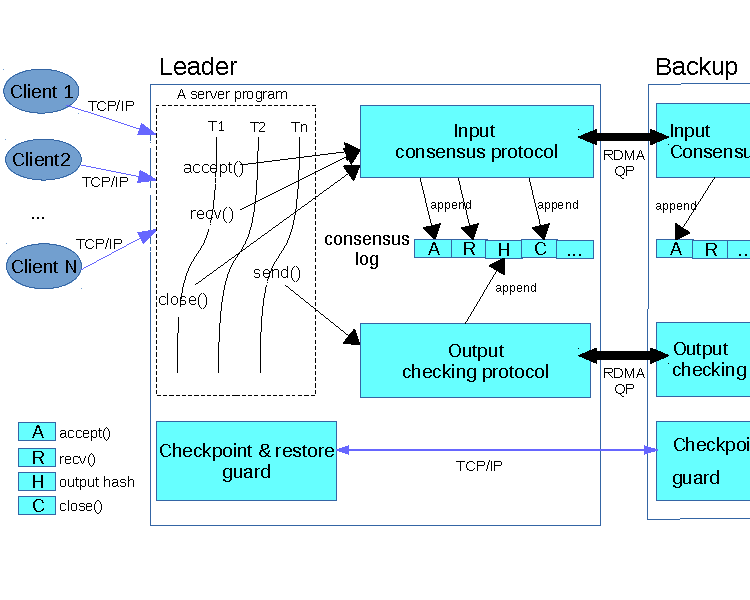
\includegraphics[width=0.5\textwidth]{figures/arch}
% \vspace{-.10in}
% \caption{{\em The \xxx Architecture.} \rm {\xxx components are shaded (and in
%   green).}} \label{fig:arch}
% \vspace{-.05in}
% \end{figure*}

% TBD. Input coordinator and output checker. Components.

% System model. Replicas. RDMA. LAN. Clients.
\xxx follows a typical \paxos runtime system 
deployment~\cite{scatter:sosp11,eve:osdi12,rex:eurosys14,crane:sosp15, 
dare:hpdc15}. It runs replicas of a server program in a datacenter. Replicas 
connect with each other using RDMA QPs. Client programs located in LAN or WAN. 
The leader handles client requests and runs our RDMA-based \paxos protocol to 
coordinate inputs among replicas.
% If a backup receives client 
% requests, it deny the requests and reply the leader's IP.

% \xxx intercepts four types of 
% socket operations: the \accept type, the \recv type, the \send type, and the 
% \close type. 
Figure~\ref{fig:arch} shows \xxx's architecture. \xxx intercepts a server 
program's socket calls (\eg, \recv) using a Linux technique called LD\_PRELOAD. 
\xxx involves four key components: a \paxos consensus protocol for input 
coordination (in short, the \emph{coordinator}), an output checking protocol 
(the \emph{checker}), a circular in-memory consensus log (the 
\emph{log}), and a guard process that handles checkpointing and recovering a 
server's process state and file system state (the \emph{guard}).

\begin{figure}[t]
\centering
\vspace{-.15in}
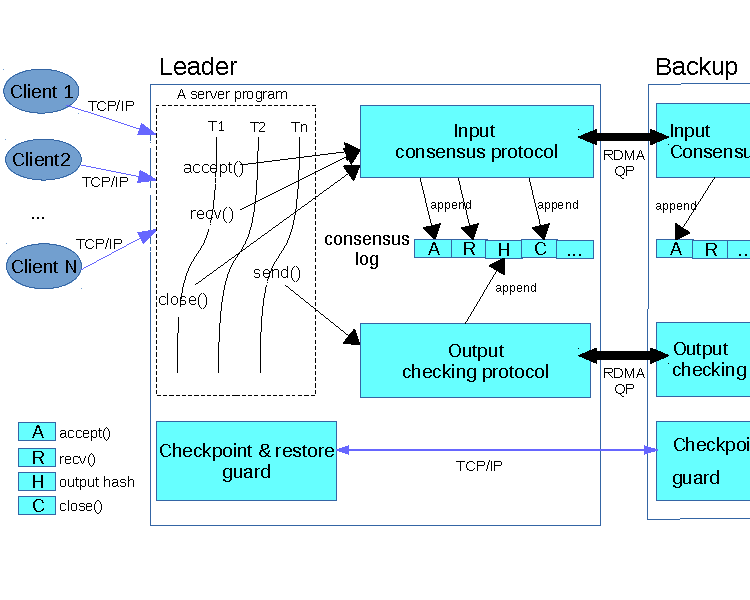
\includegraphics[width=.48\textwidth]{figures/arch}
\vspace{-.50in}
\caption{{\em The \xxx Architecture.} \xxx components are shaded (and in
  blue).}
\vspace{-.15in}
  \label{fig:arch}
\end{figure}


% Coordinator: leader side. 
The coordinator is invoked when a server program thread calls an inbound socket 
call to manage a client socket connection (\eg, \accept and \close) or to 
receive inputs from the connection (\eg, \recv). On the leader side, \xxx 
executes the actual Libc socket call, extracts the returned value or inputs of 
this call, stores it in local SSD, appends a log entry to its local consensus 
log, and then invokes the coordinator for a new consensus request on 
``executing this socket call".

The coordinator runs a consensus algorithm (\S\ref{sec:input}), which WRITEs 
the local entry to backups' remote logs in parallel and polls the local log 
entry to wait quorum. When a quorum is reached, the leader thread simply 
finishes intercepting this call and continues with its server execution. As 
the leader's server threads execute more calls, \xxx enforces the same 
consensus log and thus the same socket call sequence across replicas.

% In this request, in order tell the 
% backups what socket 
% calls they should execute, this request also carries the latest request 
% viewstamp that has reached consensus (\ie, the latest committed request).

% This coordinator invokes a consensus request by: (1) assigns this call a 
% monotonically increasing index (\ie, a viewstamp) in the log, (2) builds a 
% socket call struct (\S\ref{sec:input}), (3) store the struct to persistent 
% storage, (4) appends it to the log according to the index, and (5) writes this 
% struct to all remote backup replicas' log.

% Coordinator: backup side.
On each backup side, the coordinator uses a \xxx internal thread called 
\emph{follower} to poll its consensus log for new consensus requests. If the 
coordinator agrees the request, the follower stores the log entry in local SSD 
and then WRITEs a consensus reply to the remote leader's corresponding log 
entry. A backup does not need to intercept a server's socket calls because the 
follower will just follow the leader's consensus requests on executing what 
socket calls and then forward these calls to its local server program.

% To respond consensus requests rapidly, each 
% backup coordinator spawns a dedicated thread. This thread runs a busy loop to 
% pull consensus requests from the consensus log. This high-perfomance thread 
% runs in a spare dedicated CPU core and elinimates context switches, unlike 
% traditional TCP/IP that block threads socket calls to wait for requests.

% The backup 
% coordinator then forwards all the requests up to the latest committed socket 
% call to its local server process. 

% Consensus log. Same in both leader and backups.
% A consensus log appending operation is invoked whenever a leader's server 
% executes a socket call (except \send calls, handled by output checker). The 
% leader coordinator just appends socket calls to the log and backups follow 
% socket calls in this log.

% Output checker: leader side. % Output checker: backup side.
The output checker is occasionally invoked as the leader's server program 
executes outbound socket calls (\eg, \send). For every 1.5KB (MTU size) of 
accumulated outputs per connection, the checker unions the previous hash with 
current outputs and computes a new CRC64 hash. After a fixed number of hashes 
are generated, the checker then invokes consensus across replicas, which 
compares the hash at its global hash index on the leader side.

This output consensus is based on the input consensus algorithm 
(\S\ref{sec:input}) except that backups carry their hash at the same hash index 
back to the leader. For this particular output consensus, the leader first 
waits quorum. It then waits for a few \us in order to collect more remote 
hashes. It then compares remote hashes it has.

If a hash divergence is detected, the leader optionally invokes the local guard 
to forward a ``rollback" command to the diverged replica's guard. The diverged 
replica's guard then rolls back and restores the server program to a latest 
checkpoint before the last successful output check (\S\ref{sec:output}). The 
replica then restores and re-executes socket calls to catch up. Because output 
hash generations are fast and an output consensus is invoked occasionally, our 
evaluation didn't observe performance impact on this checker.

% Then, for every \emph{Tcheck} hash generations, the checker invokes a consensus 
% request on this hash value. This output consensus is the same as the 
% coordinator's input consensus except that backups' output checkers send ACKs 
% with their own hash values with the same index, whenever the hash values are 
% ready (some backups may run slowly). When a majority of hashes are back, the 
% leader's output checker compares these values and then makes an effort to roll 
% back divergent replicas to a previous checkpoint before the last matching hash. 


% Guard: leader side. % Guard: backup sides.
% Question: how does the backup replicas know the last matching hash? Through 
% committed viewstamp for the \send.
% The leader's guard accepts roll-back requests from the output checker and 
% forwards the requests to the corresponding guard on another, divergent repilca. 
% The divergent replca's guard then rolls back the server program to a previous 
% checkpoint before the last matching one, and then invokes the local input 
% coordinator to re-forward the requests in stable storage to the server. There 
% is no a second output hash comparisons between backups and leader until the 
% leader invokes a new output checking consensus request next time.


% \subsection{Example}\label{sec:example}
% 
% \begin{figure}[t]
% \centering
% \begin{minipage}{.5\textwidth}
% \lgrindfile{code/example.cpp.lineno}
% \end{minipage}
% \vspace{-.1in}
% \caption{{\em A server example.}} \label{fig:example}
% \vspace{-.20in}
% \end{figure}
% 
% \begin{figure}[t]
% \centering
% \begin{minipage}{.5\textwidth}
% \lgrindfile{code/client.cpp.lineno}
% \end{minipage}
% \vspace{-.1in}
% \caption{{\em A client example.}} \label{fig:client}
% \vspace{-.05in}
% \end{figure}

% TBD. A simple server with recv(), accept(), and send(). Must have a 
% concurrency bug in this toy program? Race on global var or heap?

% Describe the example code.
% Describe the example code. Describe a 'set' command from key-value store.
% Figure~\ref{fig:example} shows a simplified server code based on the \redis 
% key-value store, and Figure~\ref{fig:client} shows a client cocde. The server 
% accepts a new connection from a client, receives one input request, process the 
% request, and then sends a reply. Suppose the client sends a ``SET a b" request.

% Input coordination protocol.
% Once the client calls its \connect, the leader's server program calls the 
% \accept call intercepted by \xxx. The leader's input coordinator then invokes 
% consensus on building a new connection by writing a struct for \accept to 
% remote backups with RDMA. Once a majority of backups agree, the leader machine 
% returns from the \accept call and continues to run.

% When a client program calls its \send, leader's server traps into \xxx's \recv 
% function call, which a invokes consensus on this new input ``SET a b". If 
% a consensus is made by a majority of replicas, the leader directly returns from 
% \recv and processes the request, and each replica's dedicated thread sets up 
% a new connection to the local server because the \recv consensus request 
% notifies the backups that the last call, \accept, has reached consensus.


% Output checking protcol.
% Challenge: what if leader does more sends and replicas do fewer sends?
% When a request is processed and the server is about to send reply to the 
% client, \xxx traps into the \send call, computes historical hash value on 
% inputs when 4K bytes (MTU size). Since this request is short, no output check 
% will be invoked at this time. All backups return consensus reply to the leader 
% with their own hash values if this value is available on their replica. 
% Similarly, backups do the earlier socket call: the backups' follower forwards 
% ``SET a b" request to the local server program.

% TBD: explain why we do not need to intercept poll() function.

% TBD Question: must ask Cheng. The close logic is not clear. What do the 
% leaders and backups do for close()? Why do we have to need a NOP (if 
% backup thread does not close its connection to local server, it does not 
% matter, right)? 
% Finally, the leader's server program executes a \close call. Similarly, the 
% leader invokes consensus on this call, and the backups have this \close call in 
% their log so that they can close the 

% TBD: what is the interesting outcome of this program running with Falcon? 
% Replicating all inputs without modifications? Any chart figure/schedule? 
% Two points so far: automatically replicating all inputs without modification; 
% can tolerate one replica failure; the other two can still process requests.
% % %\section{Interface} \label{sec:example}
%TBD.
% \section{\xxx's Synchronization Wrappers for a Server} \label{sec:wrappers}

This section describes how \xxx handles a server program's 
synchronizations, including \pthread synchronizations and blocking socket 
calls. Because how to handle these synchronizations is tightly relevant 
to the \parrot \dmt scheduler we leverage, in this section, we first introduce 
some background on the \parrot scheduler, including its primitives and wrappers. 
And then we describe how \xxx leverages \parrot's primitives and wrappers to 
implement its own synchronization wrappers.

\subsection{Background: the \parrot Scheduler} \label{sec:parrot}

\begin{figure}[t]
\centering
\begin{minipage}{.5\textwidth}
\lgrindfile{code/dmt-interface.cpp}
\end{minipage}
\vspace{-.1in}
\caption{{\em The \parrot \dmt runtime's scheduler primitives.}} 
\label{fig:dmt-primitives}
\vspace{-.05in}
\end{figure}

\parrot~\cite{parrot:sosp13} is a \dmt system that uses the \ldpreload trick to 
intercept \pthread synchronizations at runtime and enforces a 
well-define, round-robin order for these operations. In this round-robin 
manner, \parrot first lets one runnable thread do one synchronization 
operation; and then, for the left runnable threads, \parrot lets the next 
thread do one synchronization operation; and then the next runnable thread, 
until all runnable threads having done one synchronization operation. Then 
\parrot repeats. To enforce this schedule, \parrot maintains a queue of runnable 
threads (\emph{run queue}) and another queue of waiting threads (\emph{wait 
queue}), like a Linux OS scheduler.

\parrot enforces an important invariant: only the thread at the head of the run 
queue can do one actual synchronization operation and manipulate the run queue 
and wait queue. After the head thread does one operation, it rotates itself 
to the tail of the run queue and wakes up the new head thread of the run queue. 
Conceptually, threads within \parrot pass a global token (the run queue head) 
around. A thread will be put into the wait queue if the synchronization object 
it requires is not available, and it will be put back to the run queue 
when this object becomes available.

\begin{figure}[t]
\centering
\begin{minipage}{.5\textwidth}
\lgrindfile{code/lock.cpp.lineno}
\end{minipage}
\vspace{-.1in}
\caption{{\em \parrot's wrapper for \mutexlock.}} 
\label{fig:lock}
% \vspace{-.05in}
\end{figure}

To implement this round-robin schedule in a compact way, \parrot provides a 
monitor-like internal interface, shown in Figure~\ref{fig:dmt-primitives}. The 
\getturn function waits until the calling thread becomes the head of the run 
queue. The \putturn function rotates the calling thread to the tail of the run 
queue and wakes up the next thread which now is the head of the run queue. The 
\wait function puts the calling thread from run queue to wait queue and blocks 
on a opaque object (\eg, a mutex or a socket descriptor), until another 
thread makes this object available and calls a \signal on this object. When a 
thread returns from a \wait function, it becomes the head of the run queue. 
Both the \wait and the \signal functions require getting the global turn.

These set of primitives are highly optimized for multi-core. Each thread has an 
integer flag and condition variable. The \getturn function spin-waits on the 
current thread's flag for a while before blocking on the condition variable. 
The \wait function needs to get the turn before it returns, so it uses the same 
combined spin- and block- wait strategy as the \getturn function. The \getturn 
and \signal functions signal both the flag and the conditional variable of the 
next thread. In common case, these operations acquire no lock and do not 
block-wait, thus the number of synchronization context switches in \parrot is 
much smaller than that in traditional \pthread synchronizations, yielding 
faster performance in \parrot than in the \pthread runtime for some 
programs~\cite{parrot:sosp13}.

% For instance, \parrot's evaluation~\cite{parrot:sosp13} showed that, when 
% transcoding an OSDI 2012 presentation video using a popular parallel transcoder 
% \mencoder, \parrot only incurred 921 context switches, while the traditional 
% Linux \pthread runtime incurred 1.9M context switches, leading to a 
% \mencoderspeedup speedup of \mencoder with \parrot.

Figure~\ref{fig:lock} shows the \mutexlock wrapper in \parrot. This wrapper 
uses try-lock to avoid deadlock: if the head of the run queue is blocked waiting 
for a lock before giving up the turn, no other thread can get the turn.

When all threads of a program block, which is common case in a server 
program, \parrot puts an internal \emph{idle thread} to the run queue, which 
simply does repetitive \getturn and \putturn operations. This idle thread 
ensures that \parrot's run queue always has threads and that \parrot's logical 
clock keeps ticking.

\parrot's blocking socket calls are nondeterministic because it 
is a \dmt system for eliminating nondeterminism in \pthread 
synchronizations. A blocking socket call's wrapper in \parrot works as 
follows. When a thread calls a blocking socket call, the thread 
calls \getturn, passes the global token to the next thread in the run 
queue, removes itself from the run queue, and then calls into the 
actual socket call. When the thread returns from the actual call, it appends 
itself to a \emph{socket queue}. Each thread at the run queue head moves the 
threads in this socket queue back to the run queue. This move-back is 
nondeterministic because threads may return from blocking socket calls 
nondeterministically and thus may be added to the socket queue in various 
orders.
% However, \parrot's invariant, only the thread at run queue 
% head can manipulate the run queue, is maintained.

\subsection{\xxx' Synchronization Wrappers for a Server}
\label{sec:socket-wrappers}

\begin{figure}[t]
\centering
\begin{minipage}{.5\textwidth}
\lgrindfile{code/check-timebubble.cpp.lineno}
\end{minipage}
\vspace{-.1in}
\caption{{\em \xxx's \checktimebubble function.}} 
\label{fig:checktimebubble}
\vspace{-.10in}
\end{figure}

\xxx wraps a rich set of common blocking socket operations, including \select, 
\poll, \epollwait, \accept, and \recv. \xxx also modifies the wrappers of 
\pthread synchronizations. These wrappers are sufficient for the server 
programs in our evaluation.

% These wrappers enforce the same logical clocks for 
% server programs' blocking operations and \pthread synchronizations across 
% different replicas and do the actual synchronization operations.

\xxx needs to modify the \mutexlock wrapper in Figure~\ref{fig:lock} to do 
three things. First, if the \paxos request sequence has been empty for a 
physical duration \ntimeout, \xxx requests a time bubble with \nclock logical 
clocks. Second, if the head of the \paxos sequence is a time bubble, \xxx 
decreases the logical clock in the time bubble by one, or it removes this bubble 
if zero clock is left. Third, \xxx signals a thread that blocks on a socket 
operation (\eg, \recv) if there is a matching client socket call (\eg, \send) at 
the head of the \paxos sequence. To do these three things, \xxx calls the 
\checktimebubble function (defined in Figure~\ref{fig:checktimebubble}) at Line 
3 of the \mutexlock wrapper in Figure~\ref{fig:lock}.

An important data structure in \xxx's wrapper is the \paxos sequence which 
contains clients' socket calls and inserted time bubbles. This sequence sits 
between the proxy and the server's processes, and it is implemented with 
Boost~\cite{boost} shared memory. \xxx uses \v{lockf()} to ensure mutual 
exclusion on this sequence because the two processes may concurrently 
manipulate this sequence. For clarity, these lock and unlock operations are 
omitted in the pseudo code.

\begin{figure}[t]
\centering
\begin{minipage}{.5\textwidth}
\lgrindfile{code/recv.cpp.lineno}
\end{minipage}
\vspace{-.1in}
\caption{{\em \xxx's wrapper for \recv.}} 
\label{fig:recv}
\vspace{-.05in}
\end{figure}

\xxx also needs to modify \parrot's idle thread mechanism because sometimes 
this thread is the only thread in the run queue, and \xxx needs to frequently 
check whether a new client socket call comes or a time bubble insertion is 
needed. To do so, \xxx replaces \parrot's \getturn and \putturn primitives 
within the idle thread to be mutex lock and unlock operations, then the idle 
thread also runs the function defined in Figure~\ref{fig:checktimebubble} to 
check and insert time bubbles.

% Introduce the poll wrapper. This is tricky because instead of letting 
% Unlike \parrot, \xxx's blocking socket calls of a server program across 
% replicas can be scheduled at consistent logical times with the \paxos sequence 
% of client socket calls and the inserted time bubbles. 

Figure~\ref{fig:recv} shows \xxx's wrapper for the \recv call. This wrapper 
ensures that the \recv calls of server programs across replicas return at 
consistent logical times. The other blocking socket calls' wrappers are 
similar. A thread calling \recv in \xxx simply calls \getturn and blocks on the 
socket descriptor using \parrot's \wait primitive. When a client 
\send call that matches this \recv becomes the head of the \paxos sequence, 
the \mutexlock wrappers wakes up the server thread blocking on \recv with the
\signal call at Line 9 in Figure~\ref{fig:checktimebubble}. The waken up thread 
dequeues a number of matching \send calls from the \paxos sequence according to 
the actual bytes received. Also, for clarity, the lock and unlock operations for 
the \paxos sequence are omitted in this \recv wrapper.


\section{The Time Bubbling Technique} \label{sec:time-bubble}

\begin{figure}[t]
\centering
\includegraphics[width=.5\textwidth]{figures/time-bubble-flow}
\vspace{-.40in}
\caption{{\em The request and time bubble flow.}} \label{fig:bubbleflow}
\vspace{-.05in}
\end{figure}

Figure~\ref{fig:bubbleflow} shows the time bubbles inserted by the \timealgo 
technique. The technique groups clients' socket operations as bursts. A request 
burst can be a group of real socket requests (rectangles), or can be a time 
bubble with a fixed number of logical clocks (circles). In this figure, black 
requests are the first operation for each burst.


In a conceptual level, \xxx uses three rules to enforce the same sequence of 
logical times for socket requests (rectangles) and thus the same schedules 
across different replicas. First, \xxx uses \paxos to ensure the same 
sequence of client socket calls as well as inserted time bubbles as a 
``\paxos request sequence" for each replica, as shown in each horizontal arrow. 
Second, \xxx uses \dmt to guarantee that it only ticks logical clocks (\ie, 
schedules \pthread synchronizations or socket operations) when this 
sequence is not empty. Third, the \timealgo technique ensures that this 
sequence is not empty, otherwise it inserts a time bubble.


Figure~\ref{fig:handlebubble} shows the work flow of our \timealgo technique 
with four steps. Each replica's \dmt just waits for a physical duration 
\ntimeout, if no further requests come, (1) the \dmt requests its own proxy to 
insert a time bubble. (2) The proxy then checks whether it sees itself as the 
primary in the \paxos protocol. If so, it asks (3) the consensus component to 
invoke consensus on whether inserting this bubble; otherwise it drops this 
request. After a consensus on this bubble insertion is reached, (4) each 
machine's proxy simply inserts the bubble into the \paxos sequence, granting 
\nclock logical clocks to the \dmt scheduler.


If a server has not exhausted the logical clocks in a time bubble after 
serving current requests, \parrot's idle thread mechanism 
(\S\ref{sec:parrot}) exhausts these clocks rapidly. 
Then, the server can continue to process further requests in time.

\begin{figure}[t]
\centering
\includegraphics[width=.5\textwidth]{figures/handle-time-bubble}
\vspace{-.30in}
\caption{{\em The work flow of inserting a time bubble.}} 
\label{fig:handlebubble}
\vspace{-.1in}
\end{figure}

% Note that even given the same sequence of real socket operations, across 
% different executions, a server program running in \xxx may still run into 
% different schedules because \dmt only waits for a short amount of time (Line 5 
% in Figure~\ref{fig:lock}) and then requests time bubbles and a SIGUSR2 signal 
% across processes may get lost. However, across different machines, the servers 
% still run the same schedules because \paxos ensures that the same amount of 
% time bubbles as well as real socket requests for the \dmt schedulers across 
% replica nodes.



% \section{Implementation Details} \label{sec:impl}

\subsection{The \paxos Protocol} \label{sec:paxos}
The \paxos consensus component (\S\ref{sec:abstraction}) is a critical 
component to enforce a consistent total order of socket calls from client 
programs. Although there are already a number of open source \paxos 
implementations~\cite{concoord, zookeeper, libpaxos}, we re-implemented a \paxos 
protocol in order to incorporate our new socket-API consensus interface.

Our \paxos implementation is based on a well-known and concise 
approach~\cite{paxos:practical}. In normal case, only the primary invokes 
consensus, thus this approach reaches consensus efficiently. In exceptional 
cases such as primary restarts, a \paxos leader election 
is invoked to resolve conflicts. In \xxx, we implemented this election via 
making the primary send a heart beat message to all the backups every 
second, and if backup replicas have not receive any heart beat message for 
three seconds, these replicas start to elect a new leader. The 
leader election contains three steps~\cite{paxos:practical}: (1) backups 
proposing a new view, which is a standard \paxos two-phase 
consensus~\cite{paxos:simple}, (2) the proposer that wins the view proposing 
itself as a primary candidate, another standard \paxos two-phase consensus, and 
(3) the new leader announcing itself as the new primary.

In our implementation, each socket call from 
the client is assigned a global, monotonically increasing viewstamp (or 
\emph{global index}) to associate with each checkpoint 
(\S\ref{sec:checkpoint}). Upon consensus on a socket call, each consensus 
component persistently stores the call type, arguments, and global index into a 
Berkeley DB storage~\cite{berkeleydb} on SSD.

Although our current \paxos implementation focuses on supporting socket 
consensus interface, this \paxos protocol logic is independent of the types and 
arguments of socket operations, so our \paxos implementation can be applied 
to other types of consensus interface as well.

\subsection{Checkpoint and Restore} \label{sec:checkpoint}
To recover or add a new replica, \xxx leverages two popular open source 
tools: \criu~\cite{criu}, to checkpoint process state such as CPU registers and 
memory; and \lxc~\cite{lxc}, to checkpoint the file system state of a server 
program's current working directory and installation directory. These two 
directories are sufficient to capture files modified by the server programs in 
our evaluation.

Incorporating \lxc into \xxx has two extra practical benefits. First, the 
server process is ran within an \lxc, which provides the server the same 
and clean initial systems state and mitigates contentions on systems resources
(\eg, file descriptors) with other processes. Second, \lxc snapshots make \xxx 
easy to deploy on multiple replicas without worrying about slight differences of 
the systems environments such as kernel and library versions. We just built \xxx 
on one replica once, did a \lxc snapshot, and then copied the snapshot to 
other replicas.

A \xxx checkpoint operation contains three steps. First, \xxx 
uses \criu to checkpoint the server's process running within the \lxc 
container and dumps the checkpoint to the process's current working directory. 
\criu needs to modify systems files (\eg, ns\_last\_pid), but \lxc's 
default isolation configuration does not permit these modifications, so we 
configure \lxc to run in ``unconfined mode". Second, \xxx stops the container, 
uses ``\v{diff --text}" to generate a patch of current working directory and 
the server's installation directory against an \lxc snapshot prepared before 
any server starts. This file system checkpoint patch is incremental and 
thus efficient (\S\ref{sec:recovery}). Third, \xxx restarts the container, and 
restores the server process with \criu.

Such a \xxx checkpoint operation is done every minute on one 
backup replica without affecting the other replicas' performance. We 
explicitly design \xxx's proxy and consensus component stateless and they do not 
require checkpoints. A \xxx restore operation reverts these steps.

One main issue on checkpointing a server process is that it constantly accepts 
socket connections, but checkpointing and restoring 
TCP stacks are notoriously difficult. Our trick to avoid this difficulty is 
based on an observation: even busy server programs have some idle moments. For 
instance, consider \apache, even running with its standard performance-stress 
benchmark \ab, we observed that in some moments the server has no alive socket 
connections. Thus, during a checkpoint operation, \xxx simply checks whether the 
server has alive connections. If so, \xxx backs off for a few seconds and then 
retries until the server has no alive connections. Since checkpoint periods do 
not have to be precise, this trick runs well (\S\ref{sec:recovery}). 
% \section{Discussions}\label{sec:discuss}
% 
This section compares \xxx and \dare's protocols (\S\ref{sec:compare}), and 
discusses \xxx's limitations (\S\ref{sec:limits}) and its broad application 
areas (\S\ref{sec:apps}).

\subsection{Comparing \xxx and \dare}\label{sec:compare}

\begin{figure}[t]
\centering
\vspace{-.5in}
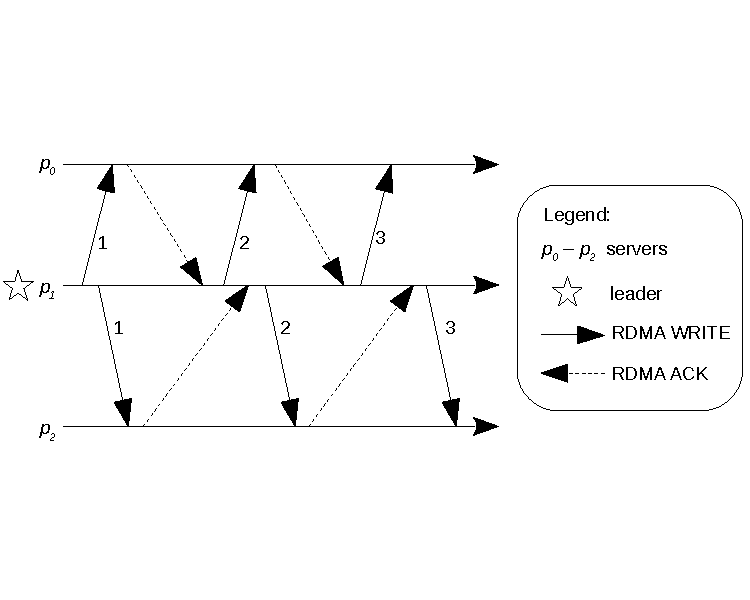
\includegraphics[width=.35\textwidth]{figures/dare}
\vspace{-.6in}
\caption{{\em \dare's RDMA-based protocol.} This is a sole-leader, 
two-round protocol with three steps: (1) the leader WRITEs a consensus request 
to all backups' consensus logs and waits for ACKs to check if they succeed; 
(2) for the successful backups in (1), leader does WRITEs to update tail 
pointer of their consensus logs; and (3) on receiving a majority of ACKs in (2), 
a consensus is reached, leader does WRITEs to notify backups without needing to 
wait ACKs.}
\label{fig:dare}
\vspace{-.20in}
\end{figure}

We highly appreciate \dare~\cite{dare:hpdc15}, the first RDMA-based, 
\paxos-like protocol. It is most relevant to \xxx. To tolerate single point of 
program failures, \dare is designed to run with a small (three to five) replica 
group. Under this design choice, \dare's protocol is sole-leader (backups do 
not participate in consensus): the leader only needs to do two-round WRITEs and 
check the ACKs of these WRITEs for a consensus. Figure~\ref{fig:dare} shows 
\dare's protocol.

% 
% logic uses two rounds to  wait for RDMA ACKs from backups. Our evaluation 
% shows that this protocol is fast when replica group size is small (three to 
% five), but both the ACK pollings and two-round

% It is a 
% sole-leader protocol (backups do not participate in consensus) with two rounds. 
% In the first round, the leader uses RDMA to write the consensus requests to all 
% replicas and polls RDMA ACKs to check whether the writes succeed. Second, for 
% the successful writes, the leader does another round of RDMA writes to mark the 
% writes as successful on other replicas, and poll ACKs on these writes. Once a 
% majority of successful writes in the second round, DARE reaches a consensus.

To further improve performance, \dare makes two technical choices. First, to 
avoid delays caused by polling ACKs, \dare uses a global RDMA CQ (Completion 
Queue) for all replicas, making it possible to collect multiple ACKs each poll 
operation. Second, this protocol does not incorporate a persistent storage or 
checkpoint/restore design. Therefore, \dare lacks durability 
(\S\ref{sec:background}), an important guarantee in traditional \paxos 
protocols and in \xxx.

% With these 
% two choices, \dare runs slightly faster than \xxx on three replicas.

However, \dare is not designed to scale to a large replica group. Our 
evaluation shows that both \dare's ACK pollings and its two-round consensus 
incurred scalability bottle approximately linearly consensus latency: DARE's 
consensus latency increased by \darescalability as replica group 
size increased by 35x (\S\ref{evaluation}).

Overall, \xxx differs from \dare in three aspects. First, \xxx is a one-round 
protocol, while \dare has two rounds. To achieve one-round consensus, \xxx's 
backups poll from its local memory to receive consensus requests, so \xxx 
consumes more CPU than \dare on backlups. Second, \xxx has shown to scale well
(sub-linearly) on 100+ nodes (\S\ref{sec:comp-dare}), while \dare did not 
discuss their scalability in paper. Third, to ensure durability, \xxx's 
protocol includes a persistent storage.

\subsection{\xxx Limitations}\label{sec:limits}

% Input coordination protocol.

% Have not hooked time and rand(). Can use PMP approach. Not a problem for 
% evaluated apps. 
\xxx currently does not hook random functions such as \v{gettimeofday()} and 
\v{rand()} because these random results are often explicit and easy to examine 
from network outputs (\eg, a timestamp in the header of a reply). Existing 
approaches~\cite{eve:osdi12,paxos:practical} in \paxos protocols can also be 
leveraged to intercept these functions and make them produce same results among 
replicas.
% because our output checkers have not detected network output 
% divergence comming from these functions

% Output checking protocol.

% Clamav style.
\xxx's output checking protocol may have false positives or false negatives, 
because it is just designed to try to improve assurance on whether replicas run 
in sync. A server program running in \xxx may have false positive when it uses 
multiple threads to serve the same client connection and uses these threads to 
concurrently add outputs (\eg, \clamav in our evaluation). 
Running a deterministic multithreading 
scheduler~\cite{coredet:asplos10,parrot:sosp13} with the server program 
addresses this problem.
% In our evaluation, all programs except \clamav uses only 
% one thread to process one client connection and they don't have such false 
% positives.

A server program may also have false negative when it triggers a software bug 
but the bug does not propagate to network outputs. From client programs' point 
of view, such bugs do not matter. Moreover, \xxx already checkpoints file 
system state to mitigate this issue.

Currently \xxx has not incorporated read-only optimization~\cite{eve:osdi12} 
because its performance overhead compared to the evaluated programs' 
unreplicated executions is already reasonable (\S\ref{sec:overhead}). However, 
\xxx can be extended to support read-only optimization if two conditions are 
met: (1) whether the semantic an operation is read-only is clear in a server 
program; and (2) the number of output bytes for this operation is fixed. GET 
requests in key-value stores often meet these two conditions.

We use GET requests to present a design. \xxx intercepts a client program's 
outbound socket calls (\eg, \send), compares the first three bytes in each call 
with ``GET". If they match, \xxx appends two extra \xxx metadata fields 
\v{read\_only} and \v{length} in this outbound call to the server. \xxx then 
intercepts a server's \recv calls and strips these two fields. If the first 
field is true, \xxx directly processes this operation in a local replica 
and strips the next \v{length} bytes from the output checker within the same
connection. In sum, \xxx processes these operations locally without making 
outputs across replicas diverge.

% When execution divergence is detected in a replica, \xxx's rollback mechanism 
% is not designed to guarantee that the re-executions of this replica will 
% definitely avoids this divergence. We made this design choice because both 
% our evaluation and a previous work Eve~\cite{eve:osdi12} found that divergence 
% happens extremely rarely in evaluation. In our evaluation, we found that simply 
% re-executing the log can practically make \xxx's replicas converge to 
% same execution states. A similar finding is that although Eve provided a 
% sequential re-execution approach to with divergence avoidance guarantee, which 
% \xxx can leverage, but even Eve's evaluation didn't experience any divergence 
% and thus this approach was not invoked.

% Read only opt?

% No guarantees on recovery. Best effort. But, can we actually server requests 
% one by one?

%% No lxc.

%% Support for Java may not be good due to the VM memory copying. Some 
% techniques that avoid memory copying may be usable~\cite{weixu:tsinghua}. Good 
% for % C/C++ programs as long as they use POSIX socket APIs.



\subsection{\xxx Has Broad Applications}\label{sec:apps}

In addition to greatly improving the availability of general server programs, 
we envision that \xxx can be applied in broad areas, and here we elaborate 
three. First, \xxx's RDMA-accelerated \paxos protocol and its implementation 
could be a template for other replication protocols (\eg, byzantine 
fault-tolerance~\cite{zyzzyva:sosp07,pbft:osdi99}). 

% Another promising direction is three-phase commit (3PC): 3PC is often 
% blamed by its intolerance on network partitions and asynchronour 
% communications, 
% and its high latency caused by the three round-trips. Fortunately, within the 
% RDMA-enabled datacenter context, people may leverage \xxx's techniques and 
% experience to build a significantly faster and more reliable 3PC protocols.

% Other replication topics.

% Parallel program analysis. Such a short coordination time can make replicas 
% run almost as fast as each other, support many time-critical analyses 
% such as race detection and security defenses.
Second, by efficiently constructing multiple, equivalent executions for the 
same program, \xxx can benefit distributed program analysis techniques. Bounded 
by the limited computing resources on single machine, recent advanced 
program analysis frameworks become 
distributed~\cite{decouple:usenix08, speck:asplos08, 
shadowreplica:ccs13, wester:parallelizing:asplos13,repframe:apsys15} in order to 
offload analyses on multiple machines. \xxx can be leveraged in these 
frameworks so that developers of analysis tools can just focus on their own 
analysis logic, while \xxx's general replication architecture handles the rest.

Moreover, program analyses developers can tightly integrate their tools with 
\xxx. For instance, they can proactively diversify the orders of socket calls 
in \xxx's consensus logs among replicas to improve replicas' tolerance on 
security attacks~\cite{con:hotpar12}.

% TBD: use \xxx to detect software bugs by checking outputs, even in 
% real-world deployments. XXX make program % inputs strongly consistent across 
% replicas, so output divergence are likely % from software bugs. XXX promising 
% 
% results in our evaluation. Find a bug in % ssdb?

% One idea: can leverage the checkpoint and rollback protocok, and the 
% consensus part, to build a system that can automatically bypass concurrency 
% bugs without fixing them. The way to bypass: proactively reordering socket 
% calls. Self-healing system.

% A core building block in future operating systems. Maintain a consistent view 
% of computing resources and data. Used in scheduling framework (Mesos) because 
% its latency is almost compatible with context switches of processes (sub 
% milli seconds).
Third, \xxx can be a core building block in the emerging datacenter operating 
systems~\cite{matei:hotcloud11, mesos:nsdi11, datacenter:os}. As a 
datacenter continuously emerges a computer, an OS may be increasingly needed for 
such a giant computer. \xxx's fast, general coordination service is especially 
suitable for such an OS's scheduler to maintain a consistent, reliable view on 
both computing resources and data in a datacenter. For instance, \xxx's 
latency is largely between less than 30 \us, much smaller than a typical 
process context switch (a few hundreds \us).

% \section{Evaluation} \label{sec:eval}

Our evaluation was done on a set of three replica machines, with each having 
Linux 3.13.0, 1Gbps bandwidth LAN, 2.80 GHz dual-socket hex-core Intel Xeon 
with 24 hyper-threading cores, 64GB memory, and 1TB SSD.

We evaluated \xxx on \nprog widely used server programs, 
including \http servers \apache~\cite{apache} and \mongoose~\cite{mongoose}; 
\clamav~\cite{clamav}, an anti-virus scanning 
server that scans files in parallel and deletes malicious ones; 
\mediatomb~\cite{mediatomb}, a \upnp multimedia server that uploads, shares, 
and transcodes pictures and videos in parallel; and \mysql~\cite{mysql}, an 
SQL database. Although \mysql has a replication 
feature~\cite{mysql:replication}, this feature is mainly for improving read 
performance, not for providing \smr fault tolerance.

\smr's high availability and fault-tolerance are attractive to these 
servers programs, because these programs provide on-line service and contain 
important in-memory execution states and storage (\eg, \clamav's 
security database, \mediatomb's SQLite~\cite{sqlite} database, and \mysql).

For \apache and \mongoose, we used \apache's own concurrency stress testing 
benchmark \ab to invoke concurrent \http requests for a PHP page, which takes 
about 70 ms for a PHP interpreter to generate the page contents. For \clamav, 
we used its own client utility \v{clamdscan} to request the server to scan 
\clamav's own source code and installation directories in parallel. For 
\mediatomb, because it has a web interface, we used \ab to invoke concurrent 
requests which use \mencoder~\cite{mencoder} to transcode a 15MB video from AVI 
to MP4. For \mysql, we used \sysbench~\cite{sysbench} to generate random select 
queries. These workloads triggered 8$\sim$12 threads in each server program to 
process requests concurrently at peak performance on our machines. These 
popular benchmarks and workloads cover CPU, network, and file-IO 
bounded operations.  

% , and they involve diverse blocking socket calls 
% (\eg, \poll, \select, \epollwait, \accept, and \recv) and intensive \pthread 
% synchronizations.

\xxx has two parameters for the \timealgo technique. The first 
parameter, $W_{timeout}$, is the physical duration that the primary's \dmt 
scheduler waits before it requests consensus on a time bubble insertion. To 
prevent this parameter significantly deferring responses, \xxx sets its 
default value 100us, two orders of magnitudes smaller than the workloads' 
response times and wide-area network latencies.

The second parameter, $N_{clock}$, is the number of logical 
clocks within each time bubble. \xxx sets its default value 1000, because we 
observed that the amounts of executed \pthread synchronizations to process each 
request in most of the evaluated servers are closed to this scale. We used 
these default values in all evaluations unless explicitly specified. A 
sensitivity evaluation on these two parameters showed that their default 
values were reasonable choices (\S\ref{sec:sensitivity}).

To mitigate network latency, benchmark clients were ran within 
the replicas' LAN. Larger latency will mask \xxx's overhead. We measured each 
workload's response time as it has direct impact on users. For each data 
point, we ran 1K requests for 20 times and then picked the median value.

The rest of this section focuses on these questions:

\begin{tightenum}

\item[\S\ref{sec:ease-of-use}:] Is \xxx easy to use?

\item[\S\ref{sec:correctness}:] Compared to nondeterministic executions, does 
\xxx consistently enforce the same sequence of network outputs among replicas?

\item[\S\ref{sec:overhead}:] What is \xxx's performance overhead compared to 
nondeterministic executions?

\item[\S\ref{sec:hint}:] When the default schedules enforced by the \parrot 
\dmt scheduler are slow, how much optimization can \parrot's performance hints 
bring to \xxx?

\item[\S\ref{sec:sensitivity}:] How sensitive are the two \timealgo parameters 
to \xxx's performance?

\item[\S\ref{sec:recovery}:] How fast are \xxx's checkpoint and recovery 
components on handling replica failures?

% \item[\S\ref{sec:race}:] If some \xxx users care about data races much, how 
% does \xxx tolerate the slowdown of data race detector by deploying it on a 
% replica?

% \item[\S\ref{sec:lesson}:] What practical lessons have we learnt during the 
% case study on these server programs with \xxx?

\end{tightenum}







\subsection{Ease of Use} \label{sec:ease-of-use}

All \nprog servers we evaluated were able to be transparently plugged and 
played in \xxx without modification. For \clamav, \mediatomb, and \mysql, we 
did not need to modify any line of code and they already have moderate 
performance overhead compared to the un-replicated nondeterministic executions. 
For \apache and \mongoose, the default schedules serialized parallel 
computations. For each of the two servers, we added two lines of soft barrier 
performance hints invented by \parrot~\cite{parrot:sosp13} to line up parallel 
computations as much as possible and compute efficient \dmt schedules (cf 
\S\ref{sec:hint}).

\subsection{Consistency of Network Outputs} \label{sec:correctness}

To verify whether the server programs running in different replicas maintain 
the same execution states, we compared each server program's network outputs 
logged in three replicas. Network outputs imply a server's execution states, 
including the outcomes of ad-hoc synchronizations and data races, which 
synchronization schedules can not capture. We ran the performance workloads and 
logged the order and contents of server programs' outgoing socket calls, 
including \send, \sendto, \sendmsg, \mywrite, and \pwrite. These calls are 
sufficient to capture all network outputs of the evaluated programs. We then 
used \v{diff} to compare the logs across replicas. 

We designed two experiment plans. In plan I, we ran \xxx with the 
programs. In plan II, we disabled only the \timealgo component in \xxx for 
three reasons: (1) we wanted to know whether \timealgo is needed to keep 
replicas in sync, (2) enabling \paxos made us easy to ship the same workload 
to replicas, and (3) enabling \parrot made us easy to intercepted and logged 
network outputs.

Among the \nprog programs, three server programs, \apache, \mediatomb, 
and \mongoose, used \ab to spawn workloads. In plan I, \xxx's logs from all 
three replicas had the same order and contents of outputs except physical 
times in the responded HTTP headers. In plan II, despite that we disabled only
the \timealgo component, the logs' order of responded HTTP headers and contents 
across replicas were different. Two server programs, \clamav and \mysql, 
used specific benchmarks to spawn workloads. In plan I, the logs showed that 
\xxx enforced the same network outputs. In plan II, the orders of the outputs 
across replicas were different. These experiments suggest that simply combining 
\paxos and \dmt is not sufficient to keep replicas in sync, and the \timealgo 
technique is needed.

To diagnose consistency of network outputs more concisely, we wrote a 
micro-benchmark for \apache. We used the \v{curl} utility to spawn two 
concurrent HTTP requests: a PUT request of a PHP page and a GET request on 
this page, and then we inspected the outcome of the GET request. We ran \apache 
in \xxx with this micro benchmark for 100 times and found that three replicas 
consistently reported the same GET result in each run, either ``200 OK" or 
``404 Not Found", depending on the order of the PUT and GET request arriving at 
the primary's proxy. And then we ran \apache's un-replicated 
execution for 100 times on each replica, and three replicas reported ``404 Not 
Found" for 6, 8, 11 times respectively.

\subsection{Performance Overhead in Normal Case} \label{sec:overhead}

\begin{figure}[t]
\centering
\includegraphics[width=0.5\textwidth]{figures/normalize-perf}
\vspace{-.30in}
\caption{\small {\em \xxx's performance normalized to un-replicated 
nondeterministic execution.}}
\label{fig:normalize-perf}
\end{figure}

% \begin{table}[b]
% \footnotesize
% \centering
% \vspace{-.05in}
% \begin{tabular}{lrrr}
% {\bf Program} & {\bf Percentage (\%)} \\
% \hline\\[-2.3ex]
% \apache                       & 1.14        \\
% \mongoose                       & 3.03        \\
% \clamav                                   & 20.96     \\
% \mediatomb                       & 23.76        \\
% \end{tabular}
% \vspace{-.05in}
% \caption{{\em Percentage of inserted time bubbles among all consensus 
% requests.}} 
% \label{tab:bubble-percentage}
% \end{table}

To understand the performance impact of \xxx's components, we divided \xxx's 
components into two major parts: the \dmt part ran by \parrot; and the proxy 
(with \paxos) part which enforces the same sequence of client socket 
calls across replicas. Each part ran independently without the other 
part. The proxy part represents the performance overhead of invoking \paxos 
consensus for client socket calls, and the \dmt part represents the \parrot 
\dmt scheduler's overhead.

Figure~\ref{fig:normalize-perf} shows the servers' performance running in 
\xxx normalized by their un-replicated nondeterministic executions. The mean 
overhead of \xxx for the \nprog evaluated programs is \overhead 
due to two main reasons. First, except for \mysql, which does fine-grained, 
per-table mutex and read-write locks frequently, the \dmt schedules were 
efficient on the other four servers. The reason is that \parrot's scheduling 
primitives are already highly optimized for multi-core (\S\ref{sec:parrot}). 
The proxy-only part incurred 0.82\%$\sim$3.46\% overhead, which is not 
surprising, because the number of socket calls is much smaller than 
the number of \pthread synchronizations in these programs. In short, \xxx's 
performance mainly depends on the \dmt schedules' performance.

\mediatomb incurred modest speedup because its transcoder \mencoder had 
significant speedup with \parrot. We inspected \mediatomb's micro performance 
counters with the Intel \vtune~\cite{vtune} profiling tool. When running in 
\xxx, \mediatomb only made 6.6K synchronization context switches, while in the 
\pthread runtime it made 0.9M synchronization context switches. This saving 
caused \mediatomb running with \parrot a 12.76\% speedup compared 
to its nondeterministic execution. The \parrot evaluation~\cite{parrot:sosp13} 
also observed a \mencoderspeedup speedup on the \mencoder program. 

The \timealgo technique saves most of needs on invoking consensus 
for the logical times of clients' socket operations, confirmed by the low 
frequency of inserted time bubbles in Table~\ref{tab:timebubbles}. \apache, 
\mediatomb, and \mongoose uses \ab as its benchmark, and each request contained 
a \connect, \send, and \close call. \clamav uses its own \v{clamdscan} 
benchmark, and each request contained 18 socket calls. \mysql's benchmark 
contained 6$\sim$7 socket calls for each query. The ratio of inserted 
bubbles is merely 6.12\%$\sim$33.35\%. \mediatomb had the highest ratio of time 
bubbles because it took the longest time (9,703ms) to process each 
request.

Note that the number of inserted time bubbles across replicas is the 
same within the same run of \xxx. Within different runs of \xxx, this number 
can be different because \ntimeout is a physical duration.

\begin{table}[b]
\footnotesize
\centering
\vspace{-.05in}
\begin{tabular}{lrrr}
{\bf Program} & {\bf \# client socket calls} & {\bf \# time bubbles}  & {\bf 
\%} \\
\hline\\[-2.3ex]
\apache                       & 3,000        &    450 &    13.04 \\
\clamav                                   & 18,000     &    1,173 &    6.12 \\
\mediatomb                       & 3,000        &    1,501 &    33.35 \\
\mongoose                       & 3,000        &    448 &    12.99 \\
\mysql                       & 6,750        &    573 &    7.82 \\
\end{tabular}
\vspace{-.05in}
\caption{{\em Ratio of time bubbles in all \paxos consensus 
requests.}} 
\label{tab:timebubbles}
\end{table}

\subsection{Optimization of \parrot's Performance Hints} \label{sec:hint}

\begin{figure}[t]
\centering
\includegraphics[width=0.5\textwidth]{figures/opt-hint}
\vspace{-.30in}
\caption{\small {Effects of \parrot's soft barrier performance hints.}}
\label{fig:opt-hint}
\end{figure}

In general, a \dmt schedule may be slow in some cases~\cite{parrot:sosp13, 
dthreads:sosp11}, because this schedule may \emph{serialize} some major 
computations that can run in parallel in the \pthread runtime. For instance, 
when we ran \xxx's \dmt scheduler \parrot with \apache and \mongoose, we 
observed that \parrot's default schedules serialized the PHP interpreters.

Fortunately, \parrot creates a set of easy to use, intuitive soft barrier 
hints~\cite{parrot:sosp13} which tell the \dmt runtime to switch to faster 
schedules. These hints are just ``soft" barriers; they timeout 
deterministically and can tolerate different number of concurrent incoming 
requests. They just make a (deterministic) effort to line up computations that 
tend to run in parallel. In addition, these hints can be safely ignored by the 
\parrot runtime without affecting a program's logic.

In our evaluation, we added two lines of hints for each of the \apache and 
\mongoose servers' source code, and the pattern was general: one line was 
added at the server's \v{main()} function to initialize the soft barrier, and 
the other before a PHP interpretation's start to tell the \dmt scheduler 
``these are the major computations to line up". The performance optimization 
effects of these hints are shown in Figure~\ref{fig:opt-hint}. These hints 
reduces \apache's overhead from a 424\% to 22.99\%, and \mongoose's from a 643\% 
to 5.09\%.

% In our evaluation, we added two lines of hints for each of the \apache and 
% \mongoose programs. The methodology of adding hints to these server programs 
% are similar: one line \v{soft\_barrier\_init(0,} \v{maxworkers,} 
% \v{100*maxworkers)} was added in the server's \v{main()} function to initialize 
% a soft barrier with an opaque id 0, and the estimated number of max worker 
% threads, and also the number of logical clock ``100" that each thread need to 
% wait on this soft barrier to line up with other threads. In our evaluation, the 
% \v{maxworkers} is the 8, the number of threads with peak performance of these 
% servers running on our machines. The second line \v{soft\_barrier\_wait(0);} 
% was 
% added before a worker thread starts to process a \http request, so that threads 
% can line up at this point with the other threads with the same opaque id and 
% process requests in parallel. These hints are just ``soft" barriers; 
% they timeout deterministically and can tolerate different number of concurrent 
% incoming requests; they just make a (deterministic) effort to line up 
% computations that tend to run in parallel.



\subsection{Sensitivity of Time Bubble Parameters} \label{sec:sensitivity}
\begin{figure}[t]
\centering
\includegraphics[width=0.5\textwidth]{figures/usleep-sensitivity}
\vspace{-.30in}
\caption{\small {\em \xxx's performance with different settings on \ntimeout 
(us).} Normalized with the default parameter.}
\label{fig:usleep-sensitivity}
\end{figure}

\begin{figure}[t]
\centering
\includegraphics[width=0.5\textwidth]{figures/nclock-sensitivity}
\vspace{-.30in}
\caption{\small {\em \xxx's performance with different settings on \nclock.} 
Normalized with the default parameter.}
\label{fig:nclock-sensitivity}
\end{figure}

The two parameters \ntimeout and \nclock for \timealgo have trade-off on 
performance. This trade-off also depends on each server program as well as its 
performance workload. A smaller \ntimeout means the \dmt 
scheduler can wait less time and then proceed with granted logical clocks with 
inserted time bubbles, but it also means that more time bubbles and thus more 
\paxos consensus are involved. A smaller value also means \timealgo runs 
similar to a per-request consensus approach. 
Figure~\ref{fig:usleep-sensitivity} shows \xxx's performance by only adjusting 
this parameter. \xxx's default setting got the best result for both \apache 
and \clamav, and it got the second best result for the other three programs. 

The \nclock parameter also faces trade-off on performance. A smaller value 
means that servers can exhaust clocks in a time bubble sooner, but if a server 
does lots of \pthread synchronizations to process a request, more time bubbles 
and thus more \paxos consensus are involved. 
Figure~\ref{fig:nclock-sensitivity} shows \xxx's performance by only adjusting 
this parameter. \xxx's default setting got the best result for \clamav, 
\mediatomb, and \mongoose, and the second best result for the other two 
programs.



\subsection{Checkpoint and Recovery} \label{sec:recovery}

\begin{table}[b]
\footnotesize
\centering
\vspace{-.05in}
\begin{tabular}{lrrrr}
{\bf Program} & {\bf C p (ms)} & {\bf R p (ms)} & {\bf C fs (ms)}  & {\bf R fs 
(ms)}\\
\hline\\[-2.3ex]
\apache                       & 33  & 48        &    3,069  & 237 \\
\clamav                               & 415  & 353     &    6,963  & 6,128 \\
\mediatomb                       & 17  & 27        &    2,852  & 213 \\
\mongoose                       & 15  & 31        &    1,294  & 169 \\
\mysql                       & 88  &  81       &    53,473  & 712 \\
\end{tabular}
\vspace{-.05in}
\caption{{\em Average time cost for \xxx's checkpoint and restoring 
component.} ``C p" means ``Checkpoint process", ``R p" means ``Restore 
process", ``C fs" means ``Checkpoint file system", and ``R fs" means 
``Restore file system".} 
\label{tab:checkpoint-time}
\end{table}

To handle replica failures, \xxx periodically invokes a checkpoint operation on 
one backup (\S\ref{sec:checkpoint}). Each \xxx checkpoint operation 
contains four time consuming parts: (1) using \criu to dump the state of a 
server process (and its child processes, if any); (2) stopping and restarting a 
\lxc container; (3) doing an incremental checkpoint on a server's current 
working directory and installation directory between the \lxc stop and start; 
and (4) restoring a process's state after the \lxc restart.

Table~\ref{tab:checkpoint-time} shows time costs for each process and file 
system checkpoint operation, and all are median values with 
20 runs. In sum, a process checkpoint or restore took at most 415ms, and a file 
system checkpoint or restore took less than 7s except \mysql. \mysql took about 
one minute to checkpoint its file system because \sysbench generated a large 
database in \mysql's installation directory. For each program, a file system 
restore operation took much less time than its checkpoint operation because a 
restore 
operation patches only files modified by the server program. A common \lxc stop 
and restart operation took 2$\sim$5s depending on the daemon processes' 
bootstrap progress within the container. Although each of these four steps in a 
\xxx checkpoint operation costs time, such a checkpoint is done on only one 
backup replica, its performance impact was negligible in our evaluation (the 
other replicas formed a quorum).

To evaluate the speed of \xxx's \paxos protocol on replica failure and 
recovery, we manually restarted the primary replica running a \mongoose server. 
The other two backups in the system then invoked a leader election with three 
steps (\S\ref{sec:paxos}), which took \recovertime. After 
the old primary's machine restarted, \xxx restarted the proxy and the 
consensus component, extracted the latest \mongoose checkpoint on the local 
machine and restored the \mongoose process and its file system. On the full 
restore of this \xxx instance, it received the new primary's heart beat message 
in \downgradetime and downgraded itself to a backup. Overall, both the \paxos 
leader election and the restarted old primary's self-downgrading took 
sub-seconds.

% We observed that the restored \mongoose server were able to continue to process 
% client requests normally, thanking to \criu and \lxc's robust implementation. 
% Overall, both the leader election and the restarted node's self-downgrading 
% took sub-seconds.



% \section{Related Work} \label{sec:related}


\para{Software-based consensus.} There are a rich set of
\paxos algorithms~\cite{paxos:practical,paxos,paxos:simple,paxos:complex,
epaxos:sosp13} and 
implementations~\cite{paxos:live,paxos:practical,chubby:osdi,crane:sosp15}. 
\paxos is notoriously difficult to be fast and 
scalable~\cite{ellis:thesis,manos:hotdep10,scatter:sosp11}. Since consensus 
protocols play a core role in datacenters~\cite{matei:hotcloud11, mesos:nsdi11, 
datacenter:os} and worldwide 
distributed systems~\cite{spanner:osdi12,mencius:osdi08}, a variety of study 
have been conducted to improve specific aspects of consensus protocols, 
including order commutativity~\cite{epaxos:sosp13}, 
understandability~\cite{raft:usenix14,paxos}, and verifiable reliability 
rules~\cite{modist:nsdi09,demeter:sosp11}.

% Although \xxx tightly integrates 
% RDMA features in \paxos, its implementation mostly complies with a popular, 
% practical approach~\cite{paxos:practical} for reliability. Other \paxos 
% approaches can also be leveraged in \xxx.


To make \paxos's throughput scalable (\ie, more replicas, higher throughput), 
various systems leverage \paxos as a core building block to develop advanced 
replication approaches, including partitioning program 
states~\cite{scatter:sosp11,dssmr,ssmr}, splitting consensus 
leadership~\cite{mencius:osdi08,spaxos}, and hieratical 
replication~\cite{manos:hotdep10,scatter:sosp11}. Theses approaches have shown 
to largely improve throughput. However, the core of these systems, 
\paxos, still faces an unscalable consensus 
latency~\cite{ellis:thesis,scatter:sosp11,manos:hotdep10}. By using \xxx as a 
building block, these system can scale even better.

% arious advanced replication models have been 
% developed~\cite{epaxos:sosp13,mencius:osdi08,scatter:sosp11,manos:hotdep10}. 



Three state machine replication (SMR) systems, Eve~\cite{eve:osdi12}, 
Rex~\cite{rex:eurosys14}, and Crane~\cite{crane:sosp15}, build traditional 
\paxos protocols to improve the availability of general server programs. 
Evaluation in these systems shows that SMR services incur modest overhead on 
server programs' throughput compared to their unreplicated executions. \xxx's 
consensus latency is one order of magnitude faster than traditional protocols 
(\S\ref{sec:eval-traditional}).
% If programs (\eg, key-value 
% stores) demand short request latency, \xxx  
% \xxx's (\S\ref{sec:compare}).
% These systems can leverage \xxx's general, 
% RDMA-accelerated protocol to improve latency.

% % DARE: simply use RDMA writes to do consensus on the leader side.
% To further improve consensus speed, DARE~\cite{dare:hpdc15} proposes a second 
% approach by simply replacing message passing in \paxos with one-sided RDMA 
% operations. For speed, DARE lets the leader handle a whole consensus round
% with three steps. The leader first appends a consensus request to a consensus 
% log in all remote replicas with RDMA writes. For the the successful writes with 
% ACKs, it then updates the tail pointers in remote logs and wait ACKs of these 
% updates. Finally, the leader knows that the minimum tail pointer among at 
% least a majority of replcias reach consensus.

% Two systems Rex and Eve did not provide latency evaluation; not open source.
% Two systems Calvin and Crane, we ran them with Calvin's database; we are XX 
% times faster.

% Notably, Eve~\cite{eve:osdi12} presents an execution state checking approach 
% based on their \paxos coordination service. Eve's completeness on detecting 
% execution divergence relies on whether developers have manually annotated all 
% thread-shared states in program code. \xxx's output checking approach is 
% automated (no manual code annotation is needed), and its completeness depends on 
% whether the diverged execution states propagate to network outputs. Eve and 
% \xxx's checking approaches are complementary and can be integrated.

% Two DARE limitations: first, no stable storage. second, old leader may 
% % unsafely writes to remote logs and thought it has reached a consensus.
% The second category includes DARE~\cite{dare:hpdc15}, a coordination protocol 
% that also uses RDMA to reduce latency. Part of \xxx's implementation was 
% inspired by DARE. \xxx differs from DARE in two major aspects.
% 
% The first difference is in a reliability model level. DARE's model is different 
% from standard \paxos's: DARE assumes that a replica's memory is still accessible 
% to remote replicas even if this replica's CPU fails, so that DARE's leader can 
% still write to remote backups. With this reliability model, DARE requires four 
% one-sided RDMA writes in each consensus round between the leader and a backup. 
% DARE's paper shows that the MTTF (mean time to failure) of memory and CPU are 
% similar.
% 
% \xxx's reliability model complies with standard \paxos's: memory 
% and CPU may fail, thus consensus requests must be written to stable storage. 
% \xxx requires two one-sided RDMA writes and two SSD writes on a consensus 
% round between the leader and a backup. DARE reported a $\sim$15 \us consensus 
% latency for write requests and $\sim$7 \us for read requests on a 64-byte 
% payload. \xxx's consensus latency is compatible with DARE's on a similar 
% payload size (\eg, \xxx's consensus latency for \ssdb was 14.6 \us in 
% Table~\ref{tab:consensus-latency}).

% Second, in a protocol level, DARE does pure-leader consensus in normal case 
% for efficiency. The leader writes a consensus request to remote replicas' 
% logs. If a majority of writes succeed with RDMA ACKs, the leader thinks that a 
% consensus has reached. DARE's backups do not invoke any proposal 
% number~\cite{paxos:simple} or view~\cite{paxos:practical} checking during 
% consensus.
% 
% In general, we argue that a pure-leader consensus approach is difficult to 
% guarantee safety. For instance, a leader may disconnect from the network 
% shortly (\eg, a temporary NIC error), reconnect, and then invoke 
% consensus requests. Concurrently, backups may start a leader election. It could 
% be risky that the leader's RDMA writes succeed and it ``thinks" that a 
% consensus has reached (because it handles everything of a consensus without any 
% backup involvement), but backups may have inconsistently started a leader 
% election.
% 
% Even if a backup first carefully does a check on a heartbeat timeout (or a 
% latest consensus request), it then closes the RDMA QP with this ``leader", 
% these two operations still have a vulnerable time window and the ``leader" can 
% write in between. Allowing a leader to ``think" that it has got a consensus 
% could be unsafe. This is probably why standard \paxos 
% protocols~\cite{paxos,paxos:simple,paxos:practical} must let backups do proposal 
% number of view checking rather than taking a pure-leader approach. \xxx complies 
% with standard \paxos protocol~\cite{paxos:practical}: a \xxx backup always 
% first compares its own view ID with the view ID in a consensus request, it then 
% agrees or rejects this request.

% The second difference is in an application level. DARE's evaluation used a 
% 335-line, single-threaded key-value store. \xxx aims to support general 
% programs.

% Various paxos protocols. Ours is complementary. Can be plugged into our 
% system.

% Three systems aim to provide SMR services to server programs. Eve, Rex, Dare, 
% Crane.
% Type I: Dare. Weaker durability. Four RDMA writes. We have two RDMA writes 
% plus two SSD writes. Compatible perf. Not for general server programs.

% Type II: Eve, Rex, Crane. All slow. Eve has output check, but also slow, use 
% TCP, and needs annotation.


\para{Hardware- or Network- assisted consensus.}  Three recent
systems~\cite{specpaxos:nsdi15,nopaxos:osdi16,hardware:paxos:nsdi16} leverage 
augmented network hardware or topology to improve \paxos consensus latency. 
``Consensus in a Box"~\cite{hardware:paxos:nsdi16} implemented \zookeeper's 
consensus protocol in FPGA and intensively modify its hardware TCP/IP stack for 
fast latency. It implemented a key-value store in hardware and showed similar 
consensus latency to \xxx on 3 or 5 replicas. It did not discuss or evaluate 
its scalability. Compared to this protocol, \xxx does not need to modify 
hardware, so it is easier to deploy and support general programs.

Speculative Paxos~\cite{specpaxos:nsdi15} and NOPaxos~\cite{nopaxos:osdi16} 
leverage the synchrony feature of datacenter topology to order requests, so 
they can eliminate consensus rounds if requests are not reordered or lost. 
Moreover, NOPaxos assigns a global sequence ID to requests so that it can 
proactively detect reordered or lost packets. If packets are lost or 
reordered, they invoke consensus to rescue. These two systems are not designed 
for scalability because when replica group becomes large, the probability that 
replicas incur ordered or lost requests may increase. Moreover, their consensus 
modules go through TCP/IP and have high round-trip latency, and \xxx can help.

\para{RDMA-based techniques.} RDMA techniques have been implemented in various 
architectures, including Infiniband~\cite{infiniband}, RoCE~\cite{roce}, and 
iWRAP~\cite{iwrap}. RDMA have been leveraged in many systems to improve 
application-specific latency and throughput, including high performance 
computing~\cite{openmpi}, key-value 
stores~\cite{pilaf:usenix14,herd:sigcomm14,farm:nsdi14,memcached:rdma}, 
transactional processing systems~\cite{drtm:sosp15,farm:sosp15}, and file 
systems~\cite{gibson:nfs}. These systems are largely complementary to \xxx. It 
will be interesting to investigate whether \xxx can improve the availability for 
both the client and server for some of these advanced systems within a 
datacenter, and we leave it for future work.

% \xxx's deployment model is to 
% provide SMR fault-tolerance to general server programs deployed in datacenters, 
% and the client programs access these server programs in LAN or WAN. 

% We didn't evaluate these systems because they are not available on client sides.


% Increasing assurance of replicas on thread schedulings. Not general 
% as Falcon's checkpoint techniques. But complementary for example ClamAV.
% \para{Nondeterminism.} 
% Nondeterminism~\cite{racepro:sosp11,dmp:asplos09,coredet:asplos10,
% cui:tern:osdi10, kendo:asplos09,
% dthreads:sosp11,peregrine:sosp11,parrot:sosp13,determinator:osdi10} is 
% pervasive in both application programs and OS kernels, and it often comes with 
% concurrency bugs~\cite{lu:concurrency-bugs}. To mitigate nondeterminism, 
% deterministic multithreading techniques~\cite{grace:oopsla09, 
% dthreads:sosp11, 
% determinator:osdi10,dpj:oopsla09, 
% dmp:asplos09,kendo:asplos09,coredet:asplos10,dos:osdi10,ddos:asplos13,
% ics:oopsla13} and deterministic replay 
% techniques~\cite{r2:osdi,friday2007,srinivasan:flashback,revirt,dejavu,
% vmware-record-replay,smp-revirt:vee08,pres:sosp09,scribe:sigmetrics10,
% odr:sosp09, capo:asplos09} have been developed. Much of these techniques can 
% greatly improve software reliability, but they often come with a performance 
% slowdown. \xxx can run these techniques with the server program to mitigate 
% replica divergence caused by concurrency bugs. 

% \para{Concurrency.} Pervasive in real-world applications. Threads. Processes. 
% Break SMR's state machine assumption. complementary.
% \para{Concurrency.} \xxx are mutually beneficial with much prior work on 
% concurrency error 
% detection~\cite{yu:racetrack:sosp,savage:eraser,racerx:sosp03,lu:muvi:sosp,
% avio:asplos06,conmem:asplos10},
% diagnosis~\cite{racefuzzer:pldi08,ctrigger:asplos09,atomfuzzer:fse08}, and
% correction~\cite{dimmunix:osdi08,gadara:osdi08,wu:loom:osdi10,cfix:osdi12}. 
% On one hand, these techniques can be deployed in \xxx's backups and help 
% \xxx detect data races. On the other hand, \xxx's asynchronous replication 
% architecture can mitigate the performance overhead of these powerful 
% analyses~\cite{repframe:apsys15}.



% \section{Conclusion}\label{sec:conclusion}

We have presented \xxx, a fast, general state machine replication system 
through building an RDMA-accelerated \paxos protocol to efficiently coordinate 
replica inputs. On top of this protocol, \xxx introduces an automated, 
efficient output checking protocol to detect and recover execution divergence 
among replicas and improve the assurance of sync in replicas. Evaluation on 
widely used, diverse server programs shows that \xxx supports these unmodified 
programs with reasonable performance overhead, and can recover from replica 
divergence caused by real-world software bugs. \xxx has the potential to 
greatly increase the adoption of state machine replication and improve the 
reliability of general programs.

% \section*{Acknowledgments}

We thank Marcos K. Aguilera (our shepherd), Yinzhi Cao, Adrian Tang, David 
Williams-King, and anonymous reviewers for their many helpful comments. This 
work was supported in part by AFRL FA8650-11-C-7190 and FA8750-10-2-0253; ONR 
N00014-12-1-0166; NSF CCF-1162021, CNS-1054906; an NSF CAREER award; an AFOSR 
YIP award; and a Sloan Research Fellowship.


\end{sloppypar}

% uncomment to tweak with bib spacing
%\setlength\bibsep{2.25pt}
{
%\small
 \bibliographystyle{abbrvnat}
 \bibliography{bib/biblio}
}

\end{document}
